% ============================================================================
% MEMORIA TFG - SemanticFIB: Buscador Semantico Inteligente para la FIB
% Version 3 (revisada y ampliada)
% Autor: Giancarlo Morales Munoz
% Director: Ramon Sanguesa
% Facultat d'Informatica de Barcelona (FIB) - UPC
% ============================================================================

\documentclass[12pt, a4paper, twoside]{report}

% --- Encoding & Language ---
\usepackage[utf8]{inputenc}
\usepackage[T1]{fontenc}
\usepackage[spanish,es-noshorthands]{babel}

% --- Fonts ---
\usepackage{lmodern}

% --- Page geometry ---
\usepackage[
  top=2.5cm,
  bottom=2.5cm,
  left=3cm,
  right=2.5cm,
  headheight=15pt
]{geometry}

% --- Headers & footers ---
\usepackage{fancyhdr}
\pagestyle{fancy}
\fancyhf{}
\fancyhead[LE]{\leftmark}
\fancyhead[RO]{\rightmark}
\fancyfoot[C]{\thepage}
\renewcommand{\headrulewidth}{0.4pt}

% --- Graphics ---
\usepackage{graphicx}
\usepackage{tikz}
\usetikzlibrary{arrows.meta, positioning, shapes.geometric, fit, calc}

% --- Tables ---
\usepackage{booktabs}
\usepackage{tabularx}
\usepackage{longtable}
\usepackage{multirow}
\usepackage{array}

% --- Colors ---
\usepackage{xcolor}
\definecolor{upcblue}{RGB}{0,51,102}
\definecolor{fibblue}{RGB}{0,102,204}
\definecolor{lightgray}{RGB}{245,247,250}

% --- Code listings ---
\usepackage{listings}
\lstset{
  basicstyle=\ttfamily\small,
  breaklines=true,
  frame=single,
  backgroundcolor=\color{lightgray},
  keywordstyle=\color{upcblue}\bfseries,
  stringstyle=\color{fibblue},
  commentstyle=\color{gray}\itshape,
  numbers=left,
  numberstyle=\tiny\color{gray},
  numbersep=8pt,
  tabsize=2,
  showstringspaces=false,
}

% --- Hyperlinks ---
\usepackage[
  colorlinks=true,
  linkcolor=upcblue,
  citecolor=upcblue,
  urlcolor=fibblue
]{hyperref}

% --- Captions ---
\usepackage{caption}
\usepackage{subcaption}
\captionsetup{font=small, labelfont=bf}

% --- Lists ---
\usepackage{enumitem}

% --- Math ---
\usepackage{amsmath}
\usepackage{amssymb}

% --- Misc ---
\usepackage{float}
\usepackage{appendix}

% --- Euro symbol ---
\usepackage{eurosym}

% ============================================================================
\begin{document}

% ============================================================================
% PORTADA
% ============================================================================
\begin{titlepage}
\begin{center}

% UPC logo
\begin{tikzpicture}
  \node[draw=upcblue, line width=2pt, minimum width=4cm, minimum height=2cm, align=center, font=\Large\bfseries\color{upcblue}] {UPC};
\end{tikzpicture}

\vspace{0.5cm}

{\large\textsc{Universitat Polit\`ecnica de Catalunya}}\\[0.2cm]
{\large\textsc{Facultat d'Inform\`atica de Barcelona}}\\[0.3cm]
{\normalsize Grado en Ingenier\'ia Inform\'atica}

\vspace{1.5cm}

\rule{\textwidth}{1.5pt}\\[0.5cm]
{\Huge\bfseries\color{upcblue} SemanticFIB}\\[0.3cm]
{\Large Buscador Sem\'antico Inteligente\\para la Facultad de Inform\'atica de Barcelona}\\[0.3cm]
{\large Basado en Ontolog\'ias y Modelos de Lenguaje}\\[0.5cm]
\rule{\textwidth}{1.5pt}

\vspace{1.5cm}

{\Large\textbf{Trabajo de Fin de Grado}}

\vspace{2cm}

\begin{tabular}{rl}
  \textbf{Autor:} & Giancarlo Morales Mu\~noz \\[0.3cm]
  \textbf{Director:} & Ramon Sang\"uesa \\[0.3cm]
  \textbf{Departamento:} & Ingenier\'ia de Servicios y Sistemas\\
  & de Informaci\'on (ESSI) \\[0.3cm]
  \textbf{Especialidad:} & Ingenier\'ia del Software \\
\end{tabular}

\vfill

{\large Cuatrimestre de Oto\~no 2024--2025}\\[0.3cm]
{\normalsize Barcelona, \today}

\end{center}
\end{titlepage}

% ============================================================================
% FRONT MATTER
% ============================================================================
\pagenumbering{roman}

% --- Resumen ---
\chapter*{Resumen}
\addcontentsline{toc}{chapter}{Resumen}

Este Trabajo de Fin de Grado presenta el dise\~no, implementaci\'on y evaluaci\'on de \textbf{SemanticFIB}, un buscador sem\'antico inteligente para la Facultad de Inform\'atica de Barcelona (FIB) de la UPC. El sistema combina t\'ecnicas de \textit{Retrieval Augmented Generation} (RAG) con una ontolog\'ia de dominio formal (RDF/OWL) para ofrecer respuestas fundamentadas a las consultas de los estudiantes sobre tr\'amites, asignaturas, normativa y servicios de la facultad.

El trabajo sigue una metodolog\'ia experimental comparativa: se implementan primero dos sistemas de referencia (\textit{baselines}) ---b\'usqueda l\'exica BM25 y b\'usqueda vectorial pura--- y, sobre ellos, se construyen y eval\'uan tres estrategias progresivamente m\'as sofisticadas: expansi\'on ontol\'ogica de consultas, b\'usqueda guiada por ontolog\'ia con vinculaci\'on de entidades y re-ranqueo controlado, y una fusi\'on h\'ibrida mediante \textit{Reciprocal Rank Fusion} (RRF). Todas las estrategias se eval\'uan de forma autom\'atica y reproducible sobre un banco de 40 consultas reales con m\'etricas est\'andar de recuperaci\'on de informaci\'on (Hit@k, MRR, nDCG).

Los resultados muestran que la expansi\'on de consultas por s\'i sola apenas mejora la b\'usqueda vectorial, mientras que la estrategia controlada ---que explota el conocimiento estructurado de la ontolog\'ia para inyectar p\'aginas can\'onicas y re-ranquear candidatos--- alcanza un \textbf{92,5\% de Hit@5 y un MRR de 0,82}, multiplicando por m\'as de dos los resultados de los \textit{baselines} y generalizando correctamente a consultas no vistas durante el dise\~no.

El resultado es un sistema funcional, desplegable localmente sin dependencias externas de pago, que proporciona respuestas precisas con citaci\'on de las fuentes originales.

\textbf{Palabras clave:} b\'usqueda sem\'antica, ontolog\'ias, RDF, OWL, SPARQL, RAG, modelos de lenguaje, recuperaci\'on de informaci\'on, BM25, ChromaDB, web scraping, FIB, UPC.

\vspace{1cm}

\chapter*{Abstract}
\addcontentsline{toc}{chapter}{Abstract}

This Bachelor's Thesis presents the design, implementation, and evaluation of \textbf{SemanticFIB}, an intelligent semantic search engine for the Barcelona School of Informatics (FIB) at UPC. The system combines Retrieval Augmented Generation (RAG) techniques with a formal domain ontology (RDF/OWL) to provide grounded answers to student queries about procedures, courses, regulations, and faculty services.

The work follows a comparative experimental methodology: two baselines are implemented first ---BM25 lexical search and pure vector search--- and three increasingly sophisticated strategies are built and evaluated on top of them: ontology-based query expansion, ontology-guided retrieval with entity linking and controlled reranking, and a hybrid fusion via Reciprocal Rank Fusion (RRF). All strategies are evaluated automatically and reproducibly on a benchmark of 40 real queries using standard information retrieval metrics (Hit@k, MRR, nDCG).

Results show that query expansion alone barely improves vector search, while the controlled strategy ---which exploits the structured knowledge of the ontology to inject canonical pages and rerank candidates--- achieves \textbf{92.5\% Hit@5 and 0.82 MRR}, more than doubling baseline performance and generalizing correctly to queries unseen during design.

\textbf{Keywords:} semantic search, ontologies, RDF, OWL, SPARQL, RAG, language models, information retrieval, BM25, ChromaDB, web scraping, FIB, UPC.

% --- Agradecimientos ---
\chapter*{Agradecimientos}
\addcontentsline{toc}{chapter}{Agradecimientos}

Quiero agradecer a mi director de TFG, Ramon Sang\"uesa, por su orientaci\'on y apoyo durante todo el proyecto. Tambi\'en a la Facultad de Inform\'atica de Barcelona por proporcionar el entorno acad\'emico y los recursos necesarios para el desarrollo de este trabajo, y a los compa\~neros que dedicaron parte de su tiempo a probar el sistema y darme su opini\'on sincera.

% --- Indices ---
\tableofcontents
\listoffigures
\listoftables

% --- Lista de acronimos ---
\chapter*{Lista de Acr\'onimos}
\addcontentsline{toc}{chapter}{Lista de Acr\'onimos}

\begin{tabular}{ll}
\textbf{ABox} & Assertional Box (instancias de una ontolog\'ia) \\
\textbf{API} & Application Programming Interface \\
\textbf{BM25} & Best Matching 25 (funci\'on de ranking l\'exico) \\
\textbf{CSS} & Cascading Style Sheets \\
\textbf{FIB} & Facultat d'Inform\`atica de Barcelona \\
\textbf{GEI} & Grau en Enginyeria Inform\`atica \\
\textbf{HTML} & HyperText Markup Language \\
\textbf{IR} & Information Retrieval \\
\textbf{LLM} & Large Language Model \\
\textbf{MRR} & Mean Reciprocal Rank \\
\textbf{nDCG} & Normalized Discounted Cumulative Gain \\
\textbf{NLP} & Natural Language Processing \\
\textbf{OWL} & Web Ontology Language \\
\textbf{PDF} & Portable Document Format \\
\textbf{RAG} & Retrieval Augmented Generation \\
\textbf{RDF} & Resource Description Framework \\
\textbf{RRF} & Reciprocal Rank Fusion \\
\textbf{SKOS} & Simple Knowledge Organization System \\
\textbf{SPARQL} & SPARQL Protocol and RDF Query Language \\
\textbf{SUS} & System Usability Scale \\
\textbf{TBox} & Terminological Box (esquema de una ontolog\'ia) \\
\textbf{TFG} & Trabajo de Fin de Grado \\
\textbf{TTL} & Turtle (serializaci\'on de RDF) \\
\textbf{UPC} & Universitat Polit\`ecnica de Catalunya \\
\textbf{URI} & Uniform Resource Identifier \\
\end{tabular}

% ============================================================================
% MAIN MATTER
% ============================================================================
\cleardoublepage
\pagenumbering{arabic}

% ============================================================================
\chapter{Introducci\'on}
\label{ch:introduccion}
% ============================================================================

\section{Contexto}

La Facultat d'Inform\`atica de Barcelona (FIB) de la Universitat Polit\`ecnica de Catalunya (UPC) es uno de los centros de referencia en formaci\'on inform\'atica en Catalu\~na y Espa\~na. Con m\'as de 3.000 estudiantes activos, m\'ultiples grados y m\'asters, centenares de asignaturas y una variedad notable de tr\'amites acad\'emicos, la cantidad de informaci\'on disponible para los estudiantes es enorme y, sobre todo, dispersa.

Cualquier estudiante de la facultad ha vivido la situaci\'on: quieres saber si quedan plazas libres en una asignatura, o cu\'ando abre el per\'iodo de matr\'icula, o qu\'e prerrequisitos tiene PROP, y acabas saltando entre cinco o seis p\'aginas de la web, el Rac\'o, alg\'un PDF de normativa y, si la cosa se complica, la cola de secretar\'ia. La informaci\'on existe ---la web de la FIB es completa y se mantiene actualizada--- pero el camino hasta ella no siempre es evidente, especialmente cuando uno no conoce el vocabulario ``oficial'' con el que est\'a etiquetada.

Este desajuste entre c\'omo pregunta un estudiante (``\textit{em vull apuntar a les assignatures}'') y c\'omo est\'a organizada la informaci\'on (``Matr\'icula > Estudiants de grau > Per\'iodes'') es, en el fondo, un problema cl\'asico de recuperaci\'on de informaci\'on con vocabulario desalineado, y es el problema que este trabajo intenta resolver.

\section{Motivaci\'on}

Los avances recientes en modelos de lenguaje (LLMs) y b\'usqueda sem\'antica ofrecen una oportunidad \'unica para crear herramientas que permitan a los estudiantes obtener respuestas r\'apidas, precisas y fundamentadas. Sin embargo, el uso directo de un LLM presenta un problema fundamental: las \textbf{alucinaciones}. Un modelo gen\'erico puede inventar informaci\'on sobre la FIB que suene convincente pero sea incorrecta; en un contexto donde la respuesta puede afectar a la matr\'icula o a un tr\'amite con plazos, esto es inaceptable.

La t\'ecnica de \textit{Retrieval Augmented Generation} (RAG) mitiga este problema combinando la capacidad generativa de los LLMs con un sistema de recuperaci\'on de documentos que ancla las respuestas en informaci\'on real y verificable. Pero el RAG tiene su propio tal\'on de Aquiles, que descubr\'i muy pronto durante el desarrollo: \textbf{la calidad de la respuesta final depende casi por completo de la calidad de la recuperaci\'on}. Si los documentos que llegan al modelo no son los correctos, ninguna habilidad generativa puede salvar la respuesta.

Por eso este TFG no trata simplemente de ``montar un chatbot RAG'', sino de estudiar de forma sistem\'atica \textbf{c\'omo mejorar la fase de recuperaci\'on usando conocimiento estructurado del dominio} ---una ontolog\'ia--- y de medir con rigor cu\'anto aporta cada mecanismo.

\section{Hip\'otesis y preguntas de investigaci\'on}

La hip\'otesis central del trabajo es que, en un dominio cerrado y bien estructurado como el de una facultad universitaria, \textbf{el conocimiento expl\'icito del dominio (ontolog\'ia) puede mejorar significativamente la recuperaci\'on sem\'antica} respecto a los enfoques puramente estad\'isticos (embeddings) o l\'exicos (BM25).

De esta hip\'otesis se derivan tres preguntas concretas que la evaluaci\'on del Cap\'itulo~\ref{ch:evaluacion} intenta responder:

\begin{enumerate}
  \item \textbf{P1:} ?`Mejora la recuperaci\'on el simple hecho de expandir la consulta con sin\'onimos y t\'erminos relacionados de la ontolog\'ia?
  \item \textbf{P2:} ?`Qu\'e aporta una integraci\'on m\'as profunda de la ontolog\'ia (vinculaci\'on de entidades, p\'aginas can\'onicas, re-ranqueo guiado) frente a la expansi\'on simple?
  \item \textbf{P3:} ?`Es preferible una fusi\'on h\'ibrida de se\~nales (l\'exica + vectorial + ontol\'ogica) o una \'unica estrategia dominante?
\end{enumerate}

Adelanto aqu\'i, porque condiciona la estructura de la memoria, que la respuesta a P1 result\'o ser esencialmente negativa, y que ese resultado ---inesperado para m\'i al principio--- fue el que reorient\'o el dise\~no del sistema hacia la estrategia de re-ranqueo controlado que acab\'o siendo la contribuci\'on principal del trabajo.

\section{Objetivos del proyecto}

El objetivo principal de este TFG es dise\~nar, implementar y evaluar un buscador sem\'antico inteligente para la FIB que:

\begin{enumerate}
  \item Recupere informaci\'on real y actualizada de la web de la FIB.
  \item Modele el dominio acad\'emico mediante una ontolog\'ia formal (RDF/OWL) poblada de forma semiautom\'atica a partir de los propios datos de la web.
  \item Implemente y compare m\'ultiples estrategias de recuperaci\'on: \textit{baselines} l\'exico y vectorial, expansi\'on ontol\'ogica, b\'usqueda controlada por ontolog\'ia y fusi\'on h\'ibrida.
  \item Eval\'ue las estrategias de forma autom\'atica y reproducible con m\'etricas est\'andar de IR sobre un banco de consultas reales.
  \item Genere respuestas naturales basadas exclusivamente en documentos verificados, citando las fuentes originales.
  \item Funcione localmente sin dependencias de servicios de pago externos.
\end{enumerate}

\section{Alcance}

El proyecto cubre el ciclo completo: desde la adquisici\'on de datos (\textit{web scraping} de \texttt{fib.upc.edu}), pasando por el procesamiento e indexaci\'on (limpieza, deduplicaci\'on, \textit{chunking}, \textit{embeddings}, ChromaDB), la modelizaci\'on del dominio (ontolog\'ia RDF/OWL con poblaci\'on semiautom\'atica), la implementaci\'on de cinco estrategias de recuperaci\'on comparables, la evaluaci\'on cuantitativa, y la interfaz de usuario (Streamlit) con generaci\'on de respuestas (LLM local).

Quedan fuera del alcance la integraci\'on con sistemas internos de la UPC (Rac\'o, eSecretaria), el soporte de datos personalizados por estudiante, y el despliegue en producci\'on con m\'ultiples usuarios concurrentes; todos ellos se discuten como trabajo futuro.

\section{Estructura del documento}

La memoria se organiza de la siguiente manera:

\begin{itemize}
  \item \textbf{Cap\'itulo 2:} Conceptos clave y fundamentos te\'oricos: ontolog\'ias, embeddings, BM25, RAG y fusi\'on de rankings.
  \item \textbf{Cap\'itulo 3:} Estado del arte en buscadores sem\'anticos, RAG y RAG aumentado con grafos de conocimiento.
  \item \textbf{Cap\'itulo 4:} Identificaci\'on del problema y actores implicados.
  \item \textbf{Cap\'itulo 5:} Alcance, requisitos y riesgos.
  \item \textbf{Cap\'itulo 6:} Metodolog\'ia y herramientas.
  \item \textbf{Cap\'itulo 7:} Arquitectura del sistema.
  \item \textbf{Cap\'itulo 8:} Implementaci\'on: el grueso del trabajo, contado en el orden en que se desarroll\'o.
  \item \textbf{Cap\'itulo 9:} Evaluaci\'on y resultados.
  \item \textbf{Cap\'itulo 10:} Planificaci\'on temporal y econ\'omica.
  \item \textbf{Cap\'itulo 11:} Sostenibilidad.
  \item \textbf{Cap\'itulo 12:} Conclusiones y trabajo futuro.
\end{itemize}


% ============================================================================
\chapter{Fundamentos Te\'oricos}
\label{ch:fundamentos}
% ============================================================================

\section{Ontolog\'ias}

\subsection{Definici\'on y prop\'osito}

Una ontolog\'ia, en el contexto de la inform\'atica, es una representaci\'on formal y expl\'icita de un conjunto de conceptos dentro de un dominio y las relaciones entre ellos \cite{gruber1993}. A diferencia de un simple glosario o taxonom\'ia, una ontolog\'ia define:

\begin{itemize}
  \item \textbf{Conceptos} (clases): entidades del dominio (ej. \textit{Asignatura}, \textit{Titulaci\'on}).
  \item \textbf{Propiedades}: atributos de los conceptos (ej. \textit{c\'odigo}, \textit{recurso can\'onico}).
  \item \textbf{Relaciones}: conexiones sem\'anticas entre conceptos (ej. \textit{pertenece\_a}, \textit{tiene\_especialidad}).
  \item \textbf{Instancias}: individuos concretos de las clases (ej. la asignatura XC, el grado GEI).
  \item \textbf{Axiomas}: reglas l\'ogicas que restringen el modelo.
\end{itemize}

Una distinci\'on que resulta central en este trabajo es la separaci\'on entre el \textbf{TBox} (\textit{Terminological Box}), que contiene el esquema conceptual ---las clases y propiedades---, y el \textbf{ABox} (\textit{Assertional Box}), que contiene las afirmaciones sobre instancias concretas. Esta separaci\'on es precisamente lo que distingue una ontolog\'ia de un simple diccionario de sin\'onimos: el esquema impone una estructura sobre la que las instancias se pueblan, se validan y se consultan.

\subsection{RDF, OWL y SPARQL}

El est\'andar de facto para representar ontolog\'ias en la web sem\'antica es la pila de tecnolog\'ias del W3C:

\begin{itemize}
  \item \textbf{RDF} (\textit{Resource Description Framework}): modelo de datos basado en tripletas \textit{(sujeto, predicado, objeto)}. Todo el conocimiento se expresa como un grafo dirigido etiquetado.
  \item \textbf{RDFS y OWL} (\textit{Web Ontology Language}): vocabularios que a\~naden sem\'antica al grafo: jerarqu\'ias de clases (\texttt{rdfs:subClassOf}), tipos de propiedades (\texttt{owl:ObjectProperty}, \texttt{owl:DatatypeProperty}), dominios y rangos.
  \item \textbf{SKOS} (\textit{Simple Knowledge Organization System}): vocabulario para sistemas de organizaci\'on del conocimiento; en este trabajo se usa para las etiquetas multiling\"ues (\texttt{skos:prefLabel}, \texttt{skos:altLabel}) y las relaciones asociativas (\texttt{skos:related}).
  \item \textbf{SPARQL}: lenguaje de consulta sobre grafos RDF, an\'alogo a SQL para bases de datos relacionales. Permite recuperar subgrafos mediante patrones de tripletas.
  \item \textbf{Turtle (TTL)}: serializaci\'on textual legible de RDF, que es el formato en que se persiste la ontolog\'ia de este proyecto.
\end{itemize}

\subsection{Ontolog\'ias ligeras vs.\ formales}

Para aplicaciones de b\'usqueda sem\'antica es com\'un utilizar ontolog\'ias ligeras que capturan vocabulario y relaciones sin la complejidad de una l\'ogica descriptiva completa (como OWL-DL con razonadores). En este trabajo se adopta un punto intermedio que me parece honesto explicitar: la ontolog\'ia es \textbf{formal en su representaci\'on} (RDF/OWL, consultable con SPARQL, inspeccionable con Prot\'eg\'e) pero \textbf{ligera en su axiomatizaci\'on} (no se utiliza razonamiento l\'ogico autom\'atico, sino consultas de grafo). La justificaci\'on es pr\'actica: para el caso de uso ---enriquecer y guiar la recuperaci\'on--- la navegaci\'on del grafo es suficiente, y el coste de un razonador no aporta beneficio medible.

\subsection{Aplicaci\'on en b\'usqueda sem\'antica}

El uso de una ontolog\'ia de dominio en un sistema de b\'usqueda permite, al menos en teor\'ia:

\begin{enumerate}
  \item \textbf{Expansi\'on de consulta:} a\~nadir sin\'onimos y t\'erminos relacionados.
  \item \textbf{Desambiguaci\'on:} identificar el sentido correcto de un t\'ermino.
  \item \textbf{Vinculaci\'on de entidades:} reconocer menciones de entidades concretas (c\'odigos de asignatura, siglas de titulaciones) y resolverlas a sus recursos.
  \item \textbf{Contexto sem\'antico:} proporcionar informaci\'on estructural al LLM.
  \item \textbf{Conocimiento can\'onico:} saber cu\'al es \textit{la} p\'agina oficial de cada concepto, independientemente de su contenido textual.
\end{enumerate}

Digo ``en teor\'ia'' porque una parte importante de este TFG consiste justamente en medir cu\'ales de estos mecanismos aportan mejora real y cu\'ales no. Como se ver\'a en el Cap\'itulo~\ref{ch:evaluacion}, los resultados son menos intuitivos de lo que esperaba al empezar.

\section{Modelos de Lenguaje (LLMs)}

\subsection{Arquitectura Transformer}

Los modelos de lenguaje actuales se basan en la arquitectura Transformer \cite{vaswani2017}, que utiliza mecanismos de atenci\'on para procesar secuencias de texto de manera paralela. Esto permite capturar dependencias a larga distancia en el texto y entrenar modelos sobre corpus masivos, dando lugar a los \textit{Large Language Models} capaces de generar texto coherente y responder preguntas en lenguaje natural.

\subsection{Modelos locales vs.\ API}

Existen dos aproximaciones principales para utilizar LLMs en una aplicaci\'on:

\begin{table}[H]
\centering
\caption{Comparativa modelos locales vs.\ API}
\label{tab:llm-comparativa}
\begin{tabularx}{\textwidth}{lXX}
\toprule
\textbf{Aspecto} & \textbf{Modelo Local (Ollama)} & \textbf{API (OpenAI)} \\
\midrule
Coste & Gratuito (hardware propio) & Por token (\$0.002--\$0.06/1K) \\
Privacidad & Total (datos locales) & Datos enviados a terceros \\
Latencia & Variable (depende del hardware) & Consistente ($<$2s) \\
Calidad & Buena (Llama 3.2 3B) & Excelente (GPT-4o) \\
Disponibilidad & Offline posible & Requiere Internet \\
\bottomrule
\end{tabularx}
\end{table}

En este proyecto se utiliza por defecto Ollama con \textbf{Llama 3.2 (3B par\'ametros)} para garantizar independencia de servicios externos y coste cero, aunque el sistema permite conmutar a la API de OpenAI mediante configuraci\'on. Cabe se\~nalar que el papel del LLM en la arquitectura final es deliberadamente acotado: genera la respuesta a partir de los documentos recuperados y condensa preguntas de seguimiento, pero \textbf{no} interviene en el ranking de documentos, que es donde se concentra la contribuci\'on del trabajo.

\section{B\'usqueda L\'exica: BM25}
\label{sec:bm25}

Antes de la era de los embeddings, la recuperaci\'on de informaci\'on se basaba en la coincidencia l\'exica ponderada. \textbf{Okapi BM25} \cite{robertson2009} sigue siendo, d\'ecadas despu\'es, un \textit{baseline} extraordinariamente competitivo y es la funci\'on de ranking de motores como Elasticsearch o Lucene. Para una consulta $Q$ con t\'erminos $q_1, \dots, q_n$ y un documento $D$:

\begin{equation}
\text{BM25}(D, Q) = \sum_{i=1}^{n} \text{IDF}(q_i) \cdot
\frac{f(q_i, D) \cdot (k_1 + 1)}{f(q_i, D) + k_1 \cdot \left(1 - b + b \cdot \frac{|D|}{\text{avgdl}}\right)}
\end{equation}

donde $f(q_i, D)$ es la frecuencia del t\'ermino en el documento, $|D|$ la longitud del documento, $\text{avgdl}$ la longitud media del corpus, y $k_1$, $b$ par\'ametros de saturaci\'on y normalizaci\'on (valores est\'andar $k_1 = 1.5$, $b = 0.75$).

La intuici\'on es simple: un documento es relevante si contiene los t\'erminos de la consulta, con m\'as peso para t\'erminos raros (IDF alto) y con saturaci\'on para evitar que la repetici\'on artificiosa de un t\'ermino dispare el score. BM25 es \textbf{fuerte en coincidencias exactas} (c\'odigos, nombres propios) y \textbf{ciego a la sinonimia}: ``profesor'' y ``docent'' son t\'erminos distintos para \'el. Este perfil complementario al de los embeddings es lo que motiva los sistemas h\'ibridos.

\section{B\'usqueda Sem\'antica y Embeddings}

\subsection{Embeddings de texto}

Un \textit{embedding} es una representaci\'on num\'erica (vector) de un texto en un espacio multidimensional donde la proximidad geom\'etrica refleja la similitud sem\'antica. Formalmente:

\begin{equation}
  f: \text{Texto} \rightarrow \mathbb{R}^d
\end{equation}

donde $d$ es la dimensionalidad del espacio (384 en nuestro caso con MiniLM).

\subsection{Similitud coseno}

La similitud entre dos vectores de embedding se calcula mediante la similitud coseno:

\begin{equation}
  \text{sim}(\mathbf{a}, \mathbf{b}) = \frac{\mathbf{a} \cdot \mathbf{b}}{||\mathbf{a}|| \cdot ||\mathbf{b}||} = \frac{\sum_{i=1}^{d} a_i b_i}{\sqrt{\sum_{i=1}^{d} a_i^2} \cdot \sqrt{\sum_{i=1}^{d} b_i^2}}
\end{equation}

El rango es $[-1, 1]$, donde 1 indica vectores id\'enticos y 0 indica ortogonalidad (ninguna relaci\'on sem\'antica).

\subsection{Modelo de embeddings multiling\"ue}

Se utiliza el modelo \texttt{paraphrase-multilingual-MiniLM-L12-v2} de Sentence Transformers \cite{reimers2019}, que:

\begin{itemize}
  \item Soporta 50+ idiomas (incluidos catal\'an y castellano), algo imprescindible dado que el corpus est\'a en catal\'an pero los estudiantes preguntan indistintamente en catal\'an y castellano.
  \item Genera vectores de 384 dimensiones.
  \item Es ligero ($\sim$120MB) y r\'apido de ejecutar en CPU, lo que permite indexar y consultar en un port\'atil sin GPU dedicada.
  \item Ofrece buena calidad en tareas de similitud sem\'antica.
\end{itemize}

La contrapartida de los embeddings, que sufrimos repetidamente durante el desarrollo, es que son \textbf{d\'ebiles ante tokens fuera de vocabulario sem\'antico}: un c\'odigo de asignatura como ``XC'' o ``PROP'' apenas aporta se\~nal al vector, porque el modelo no tiene forma de saber que se refiere a una asignatura concreta de la FIB. Esta limitaci\'on motiva el m\'odulo de vinculaci\'on de entidades del Cap\'itulo~\ref{ch:implementacion}.

\section{Retrieval Augmented Generation (RAG)}

\subsection{Problema de las alucinaciones}

Los LLMs generativos tienen tendencia a producir informaci\'on plausible pero incorrecta (alucinaciones). En un contexto acad\'emico donde la precisi\'on es cr\'itica ---plazos de matr\'icula, requisitos de normativa--- esto es inaceptable.

\subsection{Arquitectura RAG}

RAG \cite{lewis2020} combina recuperaci\'on de documentos con generaci\'on de texto:

\begin{enumerate}
  \item \textbf{Retrieval:} dada una consulta, se recuperan los $k$ documentos m\'as relevantes de una base de datos.
  \item \textbf{Augmentation:} los documentos recuperados se a\~naden al contexto del LLM.
  \item \textbf{Generation:} el LLM genera una respuesta basada exclusivamente en el contexto proporcionado.
\end{enumerate}

\begin{figure}[H]
\centering
\begin{tikzpicture}[
  node distance=1.2cm,
  block/.style={rectangle, draw=upcblue, fill=upcblue!10, minimum width=3.5cm, minimum height=1cm, align=center, rounded corners=3pt},
  arrow/.style={-{Stealth[length=3mm]}, thick, color=upcblue},
]
  \node[block] (query) {Consulta\\del usuario};
  \node[block, below=of query] (embed) {Embedding\\de la consulta};
  \node[block, below=of embed] (search) {B\'usqueda vectorial\\(ChromaDB)};
  \node[block, below=of search] (docs) {Top-K documentos\\recuperados};
  \node[block, below=of docs] (llm) {LLM\\(Llama 3.2)};
  \node[block, below=of llm] (answer) {Respuesta\\fundamentada};

  \draw[arrow] (query) -- (embed);
  \draw[arrow] (embed) -- (search);
  \draw[arrow] (search) -- (docs);
  \draw[arrow] (docs) -- (llm);
  \draw[arrow] (llm) -- (answer);

  % Ontology side
  \node[block, right=3cm of query] (ont) {Ontolog\'ia\\de dominio};
  \draw[arrow, dashed] (ont) -- node[above, font=\small] {enriquecimiento} (embed);
  \draw[arrow, dashed] (ont) |- node[right, font=\small, pos=0.3] {contexto} (llm);
\end{tikzpicture}
\caption{Arquitectura RAG b\'asica con enriquecimiento ontol\'ogico. Esta fue la primera versi\'on del sistema; la versi\'on final (Figura~\ref{fig:full-architecture}) sustituye la b\'usqueda vectorial simple por un m\'odulo de recuperaci\'on con cinco estrategias conmutables.}
\label{fig:rag-architecture}
\end{figure}

\subsection{Ventajas de RAG}

\begin{itemize}
  \item \textbf{Fundamentaci\'on:} las respuestas se basan en documentos reales.
  \item \textbf{Citabilidad:} se puede indicar la fuente de cada afirmaci\'on.
  \item \textbf{Actualizaci\'on:} no es necesario reentrenar el modelo para a\~nadir informaci\'on nueva; basta re-indexar.
  \item \textbf{Transparencia:} el usuario puede verificar las fuentes citadas.
\end{itemize}

\section{Fusi\'on de rankings: Reciprocal Rank Fusion}
\label{sec:rrf}

Cuando se dispone de varios sistemas de recuperaci\'on con perfiles complementarios (l\'exico, vectorial, ontol\'ogico), una pregunta natural es c\'omo combinarlos. \textit{Reciprocal Rank Fusion} (RRF) \cite{cormack2009} es un m\'etodo simple y sorprendentemente robusto que fusiona listas rankeadas sin necesidad de calibrar los scores de cada sistema (que viven en escalas incomparables):

\begin{equation}
  \text{RRF}(d) = \sum_{s \in S} \frac{w_s}{k + \text{rank}_s(d)}
\end{equation}

donde $S$ es el conjunto de sistemas, $\text{rank}_s(d)$ la posici\'on del documento $d$ en el ranking del sistema $s$, $w_s$ un peso opcional por sistema y $k$ una constante de suavizado (el valor $k=60$ de la literatura original). La gracia de RRF es que solo usa posiciones, no scores, evitando el problema de normalizar magnitudes heterog\'eneas. Su limitaci\'on ---que comprobamos emp\'iricamente en la Secci\'on~\ref{sec:eval-hybrid}--- es que tambi\'en \textit{diluye} las se\~nales de alta precisi\'on cuando uno de los sistemas es claramente superior a los dem\'as.


% ============================================================================
\chapter{Estado del Arte}
\label{ch:estado-arte}
% ============================================================================

\section{Sistemas de Q\&A acad\'emicos}

Diversas universidades han explorado chatbots y asistentes basados en IA para atender consultas de estudiantes. La mayor\'ia utilizan aproximaciones basadas en reglas o \textit{intents} predefinidos (tipo Dialogflow), con limitaciones evidentes en la cobertura y naturalidad de las respuestas: cada pregunta nueva exige a\~nadir un \textit{intent} a mano, y cualquier formulaci\'on fuera del guion produce respuestas gen\'ericas.

Los sistemas m\'as recientes incorporan modelos de lenguaje, pero a menudo sin mecanismos de fundamentaci\'on (\textit{grounding}) que garanticen la precisi\'on en el dominio espec\'ifico, lo que los hace vulnerables a alucinaciones sobre normativas o plazos concretos.

\section{RAG aumentado con conocimiento estructurado}

La idea de combinar recuperaci\'on neuronal con conocimiento estructurado ha ganado tracci\'on en los \'ultimos a\~nos y conviene situar este TFG dentro de esa l\'inea:

\begin{itemize}
  \item \textbf{GraphRAG} \cite{edge2024graphrag} (Microsoft) construye autom\'aticamente un grafo de conocimiento a partir del corpus mediante LLMs y lo usa para responder preguntas globales que requieren agregaci\'on. Es la referencia m\'as visible del paradigma, aunque su coste de construcci\'on (m\'ultiples pasadas de LLM sobre todo el corpus) es elevado.
  \item \textbf{KAPING} \cite{baek2023kaping} inyecta tripletas de un grafo de conocimiento directamente en el prompt del LLM, sin reentrenamiento, mejorando la factualidad en preguntas sobre entidades.
  \item \textbf{Query expansion cl\'asica con ontolog\'ias} \cite{bhogal2007review}: la expansi\'on de consultas con tesauros y ontolog\'ias es una t\'ecnica veterana de IR, con resultados hist\'oricamente mixtos: funciona cuando la expansi\'on es precisa y perjudica cuando introduce ruido ---un antecedente directo del resultado negativo que obtenemos en P1.
\end{itemize}

\section{Posicionamiento de SemanticFIB}

Frente a estos trabajos, SemanticFIB se posiciona en un nicho concreto y deliberadamente acotado:

\begin{enumerate}
  \item \textbf{Ontolog\'ia de dominio espec\'ifica y curada}, poblada semiautom\'aticamente desde la web institucional, en lugar de un grafo extra\'ido autom\'aticamente por LLMs (m\'as barato, m\'as controlable, y adecuado para un dominio peque\~no y estable).
  \item \textbf{La ontolog\'ia act\'ua en la fase de recuperaci\'on} (expansi\'on, vinculaci\'on de entidades, re-ranqueo), no solo como contexto del prompt.
  \item \textbf{Evaluaci\'on comparativa sistem\'atica} de cinco estrategias sobre el mismo corpus y el mismo banco de consultas, con divisi\'on dev/test para controlar el sobreajuste de las reglas.
  \item \textbf{100\% local y reproducible}: sin suscripciones, sin enviar datos a terceros.
  \item \textbf{Dominio acad\'emico catal\'an/castellano}, con los retos multiling\"ues que implica.
\end{enumerate}

\begin{table}[H]
\centering
\caption{Comparativa de frameworks y herramientas relacionadas}
\label{tab:rag-frameworks}
\begin{tabularx}{\textwidth}{lXccc}
\toprule
\textbf{Herramienta} & \textbf{Descripci\'on} & \textbf{Local} & \textbf{Ontolog\'ia} & \textbf{Gratuito} \\
\midrule
LangChain & Framework orquestaci\'on LLM & Parcial & No & S\'i \\
LlamaIndex & Indexaci\'on y RAG & Parcial & Parcial & S\'i \\
Haystack & Pipeline NLP completo & Parcial & No & S\'i \\
GraphRAG & Grafo autoconstruido + RAG & Parcial & Autom\'atica & S\'i \\
\textbf{SemanticFIB} & \textbf{RAG + ontolog\'ia de dominio formal} & \textbf{S\'i} & \textbf{S\'i (RDF/OWL)} & \textbf{S\'i} \\
\bottomrule
\end{tabularx}
\end{table}


% ============================================================================
\chapter{Identificaci\'on del Problema}
\label{ch:problema}
% ============================================================================

\section{Problem\'atica actual}

Los estudiantes de la FIB se enfrentan a diversas dificultades para acceder a informaci\'on acad\'emica:

\begin{itemize}
  \item Informaci\'on dispersa en m\'ultiples secciones de la web.
  \item Navegaci\'on compleja con estructuras profundas (hasta 5--6 niveles de men\'u).
  \item Vocabulario t\'ecnico-administrativo que no coincide con el vocabulario del estudiante.
  \item P\'aginas cr\'iticas (horarios, ex\'amenes, plazas libres) con muy poco texto est\'atico, dif\'iciles de encontrar por b\'usqueda de contenido.
  \item Horarios limitados de atenci\'on presencial en secretar\'ia.
  \item Falta de un punto \'unico de acceso a toda la informaci\'on.
\end{itemize}

Vale la pena detenerse en el cuarto punto, porque no era obvio al inicio del proyecto y acab\'o condicionando el dise\~no: muchas de las p\'aginas que un estudiante m\'as necesita (los horarios, el calendario de ex\'amenes, las plazas libres) son p\'aginas cuyo contenido \'util se genera din\'amicamente o se presenta en tablas, de modo que su texto indexable es m\'inimo. Cualquier sistema basado puramente en similitud de contenido las penaliza, justo al rev\'es de lo que el usuario espera.

\section{Actores implicados}

\begin{table}[H]
\centering
\caption{Actores del sistema y sus intereses}
\label{tab:actores}
\begin{tabularx}{\textwidth}{lX}
\toprule
\textbf{Actor} & \textbf{Inter\'es} \\
\midrule
Estudiantes de grado & Acceder r\'apidamente a informaci\'on sobre asignaturas, matr\'icula, tr\'amites \\
Estudiantes de m\'aster & Consultar normativa espec\'ifica, movilidad, TFM \\
Futuros estudiantes & Notas de corte, planes de estudios, proceso de acceso \\
Personal de secretar\'ia & Reducir consultas repetitivas, liberar tiempo \\
Profesorado & Derivar alumnos a informaci\'on oficial \\
Equipo directivo & Mejorar la satisfacci\'on de los estudiantes \\
\bottomrule
\end{tabularx}
\end{table}

\section{Soluci\'on propuesta}

SemanticFIB aborda este problema proporcionando:

\begin{itemize}
  \item Un punto \'unico de acceso conversacional.
  \item Comprensi\'on sem\'antica de las consultas (no solo palabras clave), reforzada con conocimiento expl\'icito del dominio.
  \item Respuestas fundamentadas con fuentes verificables.
  \item Tratamiento espec\'ifico de las p\'aginas can\'onicas de bajo contenido textual.
  \item Disponibilidad 24/7 sin coste operativo.
\end{itemize}


% ============================================================================
\chapter{Alcance del Proyecto}
\label{ch:alcance}
% ============================================================================

\section{Objetivos espec\'ificos}

\begin{enumerate}
  \item Implementar un scraper robusto para \texttt{fib.upc.edu} que extraiga informaci\'on estructurada.
  \item Dise\~nar una ontolog\'ia formal (RDF/OWL) del dominio acad\'emico de la FIB, poblada semiautom\'aticamente.
  \item Implementar cinco estrategias de recuperaci\'on comparables bajo una interfaz com\'un.
  \item Construir un pipeline RAG que integre ontolog\'ia, embeddings y LLM.
  \item Crear un banco de consultas etiquetado y un sistema de evaluaci\'on autom\'atica con m\'etricas de IR.
  \item Desarrollar una interfaz web usable que permita comparar las estrategias en vivo.
\end{enumerate}

\section{Requisitos funcionales}

\begin{table}[H]
\centering
\caption{Requisitos funcionales del sistema}
\label{tab:req-funcionales}
\begin{tabularx}{\textwidth}{clX}
\toprule
\textbf{ID} & \textbf{Prioridad} & \textbf{Descripci\'on} \\
\midrule
RF01 & Alta & El sistema debe responder preguntas en lenguaje natural (catal\'an y castellano) \\
RF02 & Alta & Las respuestas deben citar fuentes originales (URLs) \\
RF03 & Alta & El sistema debe funcionar sin conexi\'on a APIs de pago \\
RF04 & Alta & El sistema debe ofrecer m\'ultiples estrategias de recuperaci\'on conmutables \\
RF05 & Alta & La evaluaci\'on de las estrategias debe ser autom\'atica y reproducible \\
RF06 & Media & La ontolog\'ia debe enriquecer y guiar la recuperaci\'on \\
RF07 & Media & La interfaz debe mostrar detalles de la b\'usqueda (documentos, scores, boosts) \\
RF08 & Media & Mantener historial de conversaci\'on con condensaci\'on de preguntas de seguimiento \\
RF09 & Baja & Soportar indexaci\'on de documentos PDF adicionales \\
\bottomrule
\end{tabularx}
\end{table}

\section{Requisitos no funcionales}

\begin{table}[H]
\centering
\caption{Requisitos no funcionales}
\label{tab:req-no-funcionales}
\begin{tabularx}{\textwidth}{clX}
\toprule
\textbf{ID} & \textbf{Prioridad} & \textbf{Descripci\'on} \\
\midrule
RNF01 & Alta & Tiempo de respuesta de recuperaci\'on inferior a 2 segundos \\
RNF02 & Alta & Despliegue local sin infraestructura externa \\
RNF03 & Media & Interfaz responsive y profesional \\
RNF04 & Media & C\'odigo modular y extensible (a\~nadir una estrategia no debe tocar las dem\'as) \\
RNF05 & Media & Ampliar la cobertura de la ontolog\'ia sin modificar c\'odigo \\
RNF06 & Baja & Documentaci\'on completa del sistema \\
\bottomrule
\end{tabularx}
\end{table}

\section{Obst\'aculos y riesgos}

\begin{table}[H]
\centering
\caption{Riesgos identificados y mitigaciones}
\label{tab:riesgos}
\begin{tabularx}{\textwidth}{lclX}
\toprule
\textbf{Riesgo} & \textbf{Prob.} & \textbf{Impacto} & \textbf{Mitigaci\'on} \\
\midrule
Cambios en web FIB & Media & Alto & Selectores flexibles, m\'ultiples fallbacks \\
Calidad LLM local & Baja & Medio & Prompt engineering, restricci\'on a docs \\
Sobreajuste de las reglas al banco de consultas & Media & Alto & Divisi\'on dev/test con consultas held-out \\
Datos duplicados / ruido del scraping & Alta & Medio & Deduplicaci\'on, filtros de calidad en ingesta \\
Embeddings no multiling\"ues & Baja & Alto & Modelo MiniLM multiling\"ue (50+ idiomas) \\
\bottomrule
\end{tabularx}
\end{table}

El tercer riesgo merece comentario: cuando un sistema incorpora reglas dise\~nadas a partir del an\'alisis de errores, existe el peligro de evaluar el sistema con las mismas consultas que motivaron las reglas, infl\'andose artificialmente los resultados. Fui consciente de este riesgo a mitad del desarrollo y la mitigaci\'on (separar consultas de dise\~no y consultas held-out) se explica en la Secci\'on~\ref{sec:golden-set}.


% ============================================================================
\chapter{Metodolog\'ia y Herramientas}
\label{ch:metodologia}
% ============================================================================

\section{Metodolog\'ia de desarrollo}

Se ha seguido una metodolog\'ia \textbf{\'agil iterativa} con sprints de 2--3 semanas. Cada sprint produce un incremento funcional del sistema que puede evaluarse de forma independiente. M\'as all\'a de la planificaci\'on, el desarrollo real sigui\'o un ciclo que se repiti\'o varias veces y que estructura el Cap\'itulo~\ref{ch:implementacion}: \textit{implementar $\rightarrow$ evaluar $\rightarrow$ analizar errores $\rightarrow$ redise\~nar}. Varias de las decisiones m\'as importantes del proyecto (el re-ranqueo controlado, la vinculaci\'on de entidades, la deduplicaci\'on can\'onica) no estaban en el dise\~no inicial: surgieron del an\'alisis de fallos concretos.

\begin{figure}[H]
\centering
\begin{tikzpicture}[
  sprint/.style={rectangle, draw=fibblue, fill=fibblue!10, minimum width=2.5cm, minimum height=1.2cm, align=center, rounded corners},
  arrow/.style={-{Stealth[length=2mm]}, thick, color=fibblue},
]
  \node[sprint] (s1) {Sprint 1\\Scraping};
  \node[sprint, right=1cm of s1] (s2) {Sprint 2\\Indexaci\'on\\+ Baselines};
  \node[sprint, right=1cm of s2] (s3) {Sprint 3\\Ontolog\'ia\\+ RAG};
  \node[sprint, right=1cm of s3] (s4) {Sprint 4\\Reranking +\\H\'ibrido + UI};
  \node[sprint, right=1cm of s4] (s5) {Sprint 5\\Evaluaci\'on\\+ Memoria};

  \draw[arrow] (s1) -- (s2);
  \draw[arrow] (s2) -- (s3);
  \draw[arrow] (s3) -- (s4);
  \draw[arrow] (s4) -- (s5);
\end{tikzpicture}
\caption{Sprints del proyecto}
\label{fig:sprints}
\end{figure}

\section{Herramientas y tecnolog\'ias}

\begin{table}[H]
\centering
\caption{Stack tecnol\'ogico del proyecto}
\label{tab:stack}
\begin{tabularx}{\textwidth}{llX}
\toprule
\textbf{Componente} & \textbf{Tecnolog\'ia} & \textbf{Justificaci\'on} \\
\midrule
Lenguaje & Python 3.9+ & Ecosistema ML/NLP, productividad \\
LLM & Ollama + Llama 3.2 (3B) & Local, gratuito, buena calidad \\
Embeddings & Sentence Transformers & Multiling\"ue, ligero (120MB) \\
Vector DB & ChromaDB & Embebido, zero-config, persistente \\
B\'usqueda l\'exica & rank-bm25 & Implementaci\'on Okapi BM25 pura en Python \\
Ontolog\'ia & rdflib (RDF/OWL/SPARQL) & Est\'andar W3C, serializaci\'on Turtle \\
Orquestaci\'on & LangChain & Abstracciones RAG maduras \\
Scraping & BeautifulSoup + requests & Robusto, flexible, ligero \\
Frontend & Streamlit & Prototipado r\'apido, componentes ricos \\
Control de versiones & Git & Est\'andar de la industria \\
\bottomrule
\end{tabularx}
\end{table}

La elecci\'on de \texttt{rdflib} frente a alternativas m\'as pesadas (Apache Jena, GraphDB) responde al mismo criterio que el resto del stack: todo el sistema debe poder ejecutarse en un port\'atil sin servicios externos. \texttt{rdflib} carga el grafo en memoria (poco m\'as de mil tripletas en nuestro caso), soporta SPARQL completo y serializa a Turtle, que es todo lo que el proyecto necesita.

\section{Entorno de desarrollo}

\begin{itemize}
  \item \textbf{Sistema operativo:} macOS (Apple Silicon)
  \item \textbf{Editor:} Visual Studio Code con extensiones Python
  \item \textbf{Gestor de paquetes:} pip + entorno virtual (venv)
  \item \textbf{Inspecci\'on de la ontolog\'ia:} Prot\'eg\'e / visualizadores RDF
\end{itemize}


% ============================================================================
\chapter{Arquitectura del Sistema}
\label{ch:arquitectura}
% ============================================================================

\section{Visi\'on general}

SemanticFIB sigue una arquitectura modular con separaci\'on clara de responsabilidades. El flujo de datos tiene dos caminos: \textbf{offline} (adquisici\'on e indexaci\'on) y \textbf{online} (consulta). La diferencia m\'as importante respecto a un RAG convencional es el m\'odulo de recuperaci\'on: en lugar de una \'unica b\'usqueda vectorial, existe una \textbf{factor\'ia de estrategias} que expone cinco modos conmutables bajo la misma interfaz, lo que permite tanto la comparaci\'on experimental del Cap\'itulo~\ref{ch:evaluacion} como la selecci\'on en vivo desde la interfaz.

\begin{figure}[H]
\centering
\begin{tikzpicture}[
  node distance=1.0cm and 1.6cm,
  module/.style={rectangle, draw=upcblue, fill=upcblue!8, minimum width=3cm, minimum height=0.9cm, align=center, rounded corners=4pt, font=\small},
  data/.style={cylinder, draw=fibblue, fill=fibblue!10, minimum width=2cm, minimum height=0.9cm, align=center, font=\small, shape border rotate=90, aspect=0.3},
  arrow/.style={-{Stealth[length=2.5mm]}, thick},
  darrow/.style={-{Stealth[length=2.5mm]}, thick, dashed},
]
  % Offline pipeline (left)
  \node[module] (scraper) {Scraper\\(\texttt{scraper.py})};
  \node[data, below=of scraper] (json) {JSON\\scraped\_data};
  \node[module, below=of json] (ingest) {Ingesta: dedup +\\chunking (\texttt{ingest.py})};
  \node[module, below=of ingest] (embedder) {Embedder\\(MiniLM)};
  \node[data, below=of embedder] (chroma) {ChromaDB\\(vectores)};
  \node[data, right=1.2cm of json] (ttl) {Ontolog\'ia\\(.ttl)};
  \node[module, above=of ttl] (builder) {Constructor\\ontolog\'ia};

  \draw[arrow] (scraper) -- (json);
  \draw[arrow] (json) -- (ingest);
  \draw[arrow] (ingest) -- (embedder);
  \draw[arrow] (embedder) -- (chroma);
  \draw[arrow] (json) -- (builder);
  \draw[arrow] (builder) -- (ttl);
  \draw[darrow] (ttl) |- (ingest);

  % Online pipeline (right)
  \node[module, right=5.2cm of scraper] (ui) {Streamlit UI\\(\texttt{app.py})};
  \node[module, below=of ui] (rag) {RAG Chain\\(condensaci\'on + LLM)};
  \node[module, below=of rag] (factory) {Factor\'ia de retrievers\\(\texttt{retrieval/})};
  \node[module, below=of factory, xshift=-1.8cm, minimum width=1.6cm] (bm25) {BM25};
  \node[module, below=of factory, xshift=0cm, minimum width=1.6cm] (dense) {Dense};
  \node[module, below=of factory, xshift=1.9cm, minimum width=1.9cm] (ctrl) {Controlada\\+ h\'ibrida};

  \draw[arrow] (ui) -- (rag);
  \draw[arrow] (rag) -- (factory);
  \draw[arrow] (factory) -- (bm25);
  \draw[arrow] (factory) -- (dense);
  \draw[arrow] (factory) -- (ctrl);
  \draw[darrow] (bm25) |- (chroma);
  \draw[darrow] (dense) |- (chroma);
  \draw[darrow] (ctrl) |- (chroma);
  \draw[darrow] (ttl) -| (ctrl);

  % Labels
  \node[above=0.3cm of scraper, font=\bfseries\color{upcblue}] {Pipeline Offline};
  \node[above=0.3cm of ui, font=\bfseries\color{upcblue}] {Pipeline Online};
\end{tikzpicture}
\caption{Arquitectura completa del sistema SemanticFIB. La ontolog\'ia participa en ambos pipelines: en la ingesta (preservaci\'on de p\'aginas can\'onicas) y en la consulta (expansi\'on, entity linking, re-ranqueo).}
\label{fig:full-architecture}
\end{figure}

\section{Estructura de ficheros}

\begin{lstlisting}[language={}, caption={Estructura del proyecto}, label={lst:structure}]
semanticfib/
|-- app.py                   # Interfaz Streamlit
|-- scraper.py               # Web scraper FIB
|-- ingest.py                # Indexacion: dedup + chunking + embeddings
|-- settings.py              # Configuracion central
|-- chatbot/
|   |-- llm.py               # Configuracion LLM (Ollama/OpenAI)
|   |-- rag_chain.py         # Pipeline RAG + condensacion de preguntas
|-- db/
|   |-- vector_store.py      # Wrapper ChromaDB (upsert idempotente)
|-- ontology/
|   |-- build_ontology.py    # Construccion del grafo RDF/OWL
|   |-- fib_ontology.py      # API de consulta (matching, SPARQL)
|   |-- fib_ontology.ttl     # Serializacion Turtle (generada)
|-- retrieval/
|   |-- base.py              # Interfaz comun de resultados
|   |-- bm25.py              # Baseline lexico
|   |-- dense.py             # Baseline vectorial
|   |-- ontology_expansion.py# Expansion ontologica naive
|   |-- entity_linker.py     # Vinculacion de entidades
|   |-- controlled_ontology.py # Busqueda controlada por ontologia
|   |-- hybrid_rrf.py        # Fusion hibrida RRF
|-- evaluation/
|   |-- queries.json         # Golden set (40 consultas, dev/test)
|   |-- evaluate.py          # Evaluacion automatica (Hit@k, MRR, nDCG)
|   |-- results/             # Resultados con timestamp (CSV + JSON)
|-- processing/
|   |-- embedder.py          # Generacion embeddings
|   |-- pdf_loader.py        # Carga y chunking PDFs
|-- scraped_data/
|   |-- fib_documents.json   # Datos scrapeados
|-- chroma_db/               # Base de datos vectorial
\end{lstlisting}

\section{Flujo de datos}

\subsection{Pipeline Offline (Indexaci\'on)}

\begin{enumerate}
  \item El \textbf{Scraper} recorre \texttt{fib.upc.edu} y extrae documentos estructurados (1.812 documentos de 411 p\'aginas en la \'ultima ejecuci\'on).
  \item El \textbf{constructor de la ontolog\'ia} genera el grafo RDF a partir del esquema declarado y de los datos scrapeados (nombres oficiales de asignaturas, URLs can\'onicas).
  \item El script de \textbf{ingesta} deduplica los documentos (priorizando URLs can\'onicas), los divide en chunks respetando p\'arrafos y frases, y filtra fragmentos de bajo valor.
  \item El \textbf{Embedder} genera vectores de 384 dimensiones para cada chunk (incluyendo t\'itulo y secci\'on como contexto).
  \item \textbf{ChromaDB} almacena vectores, textos y metadatos de forma persistente e idempotente (\textit{upsert}).
\end{enumerate}

\subsection{Pipeline Online (Consulta)}

\begin{enumerate}
  \item El usuario escribe una pregunta en la interfaz.
  \item Si hay historial de conversaci\'on, el LLM \textbf{condensa} la pregunta de seguimiento en una pregunta aut\'onoma.
  \item El \textbf{retriever del modo activo} recupera los documentos m\'as relevantes (el detalle de cada estrategia se da en el Cap\'itulo~\ref{ch:implementacion}).
  \item El \textbf{LLM} genera una respuesta basada en los documentos, con el contexto ontol\'ogico como conocimiento estructurado adicional y con las fuentes citadas.
  \item La \textbf{UI} muestra la respuesta, las fuentes y los detalles t\'ecnicos (query enriquecida, entidades detectadas, boosts aplicados).
\end{enumerate}

% ============================================================================
\chapter{Implementaci\'on}
\label{ch:implementacion}
% ============================================================================

Este cap\'itulo es el n\'ucleo de la memoria y est\'a contado, deliberadamente, en el orden en que se desarroll\'o el sistema. Me parece m\'as honesto y m\'as \'util que presentar el resultado final como si hubiera nacido completo: muchas de las piezas que acabaron siendo centrales (la deduplicaci\'on can\'onica, la vinculaci\'on de entidades, el re-ranqueo controlado) no estaban en el dise\~no inicial, y entender \textit{por qu\'e} aparecieron explica mejor el sistema que cualquier descripci\'on est\'atica.

\section{Adquisici\'on de datos: Web Scraping}

\subsection{Punto de partida}

El primer sprint se dedic\'o \'integramente a la adquisici\'on de datos. La premisa del proyecto es que el sistema trabaja \textbf{\'unicamente} con informaci\'on oficial de la FIB, as\'i que todo empieza por extraer el contenido de \texttt{fib.upc.edu} y sus subp\'aginas.

El scraper implementa un recorrido BFS (\textit{breadth-first search}) a partir de la p\'agina principal, con las siguientes reglas:

\begin{itemize}
  \item Solo se siguen enlaces internos del dominio \texttt{fib.upc.edu}.
  \item Se excluyen recursos no textuales (im\'agenes, CSS, JS) y p\'aginas de login.
  \item Se respeta un retardo entre peticiones para no sobrecargar el servidor.
  \item De cada p\'agina se extraen: URL, t\'itulo, secciones (encabezados \texttt{h1--h4}) y el texto limpio de cada secci\'on.
\end{itemize}

La extracci\'on por secciones, en lugar de p\'aginas enteras, fue una decisi\'on temprana que result\'o acertada: las p\'aginas de la FIB suelen agrupar varios temas bajo encabezados distintos (por ejemplo, la p\'agina de matr\'icula tiene secciones de per\'iodos, procedimiento y documentaci\'on), y tratar cada secci\'on como documento independiente mejora la granularidad de la recuperaci\'on.

La \'ultima ejecuci\'on completa del scraper proces\'o \textbf{411 p\'aginas} y produjo \textbf{1.812 documentos} (secciones), que tras la limpieza y deduplicaci\'on de la Secci\'on~\ref{sec:ingesta} se convierten en unos \textbf{2.700 chunks} indexados.

\subsection{Problemas encontrados}

No todo fue tan directo como suena. Tres problemas concretos del scraping acabaron teniendo consecuencias en fases posteriores:

\begin{enumerate}
  \item \textbf{Contenido duplicado entre URLs distintas.} La web de la FIB publica la misma p\'agina bajo varias rutas (por idioma, por titulaci\'on, por redirecciones hist\'oricas). Por ejemplo, la p\'agina de ``places lliures'' es id\'entica para varios grados pero vive en URLs diferentes. Al principio no le di importancia; m\'as adelante (Secci\'on~\ref{sec:dedup}) result\'o ser una fuente seria de problemas.
  \item \textbf{P\'aginas din\'amicas con poco texto.} Horarios, calendarios de ex\'amenes y plazas libres generan su contenido \'util con JavaScript o tablas, de modo que el HTML est\'atico apenas contiene texto indexable. Son precisamente las p\'aginas que m\'as consultan los estudiantes.
  \item \textbf{Mezcla de idiomas.} El corpus est\'a mayoritariamente en catal\'an, pero hay secciones en castellano e ingl\'es, y los usuarios preguntan en cualquiera de los dos primeros. Esto condicion\'o la elecci\'on del modelo de embeddings multiling\"ue.
\end{enumerate}

\section{La ontolog\'ia de dominio}
\label{sec:ontologia}

\subsection{Primera iteraci\'on: un diccionario de sin\'onimos}

Mi primera aproximaci\'on a la ``ontolog\'ia'' fue, siendo sincero, un diccionario de Python: un mapa de conceptos a listas de sin\'onimos (\texttt{\{"matricula": ["matriculaci\'o", "inscripci\'o", ...]\}}) que serv\'ia para expandir las consultas. Funcionaba como prueba de concepto, pero ten\'ia tres carencias que se hicieron evidentes en cuanto el proyecto creci\'o:

\begin{enumerate}
  \item \textbf{No era una ontolog\'ia.} No hab\'ia clases, ni jerarqu\'ia, ni relaciones tipadas: solo vocabulario plano. Dif\'icilmente pod\'ia defender en la memoria que el sistema estaba ``basado en ontolog\'ias''.
  \item \textbf{No escalaba.} A\~nadir las $\sim$100 asignaturas del GEI con sus c\'odigos y URLs a mano era inviable y fr\'agil.
  \item \textbf{No era consultable.} Cualquier operaci\'on no prevista (``dame todos los conceptos relacionados con tr\'amites'') requer\'ia escribir c\'odigo nuevo en lugar de una consulta declarativa.
\end{enumerate}

\subsection{Segunda iteraci\'on: grafo formal RDF/OWL}

Despu\'es de investigar las opciones del ecosistema de la web sem\'antica (Secci\'on 2.1), redise\~n\'e la ontolog\'ia como un \textbf{grafo RDF formal} construido con \texttt{rdflib}, con esquema OWL y vocabulario SKOS, serializado en Turtle (\texttt{fib\_ontology.ttl}). La Figura~\ref{fig:tbox_abox} muestra la arquitectura en dos capas.

\begin{figure}[H]
\centering
\begin{tikzpicture}[
  node distance=1.5cm and 2cm,
  tboxnode/.style={rectangle, draw=upcblue, fill=upcblue!10, minimum width=2.5cm, minimum height=1cm, align=center, rounded corners, font=\small\bfseries},
  aboxnode/.style={ellipse, draw=fibblue, fill=fibblue!10, minimum width=2cm, align=center, font=\small},
  rel/.style={-{Stealth[length=2mm]}, thick, color=upcblue, font=\scriptsize},
  isa/.style={-{Stealth[length=2mm, open]}, thick, color=gray, dashed, font=\scriptsize}
]
  % Cajas de fondo
  \node[fill=gray!5, rounded corners, draw=gray!40, dashed, minimum width=14cm, minimum height=5cm] (tbox) at (2,-1.5) {};
  \node[anchor=north west, font=\itshape\bfseries\color{gray}] at (tbox.north west) {TBox (Esquema Conceptual)};

  \node[fill=fibblue!5, rounded corners, draw=fibblue!30, dashed, minimum width=14cm, minimum height=3.5cm] (abox) at (2,-6.5) {};
  \node[anchor=north west, font=\itshape\bfseries\color{fibblue}] at (abox.north west) {ABox (Afirmaciones de Instancias)};

  % Capa TBox (Clases)
  \node[tboxnode] (entitat) at (2,0) {EntitatAcademica};
  \node[tboxnode] (titulacio) at (-2,-2) {Titulacio};
  \node[tboxnode] (assignatura) at (2,-2) {Assignatura};
  \node[tboxnode] (especialitat) at (6,-2) {Especialitat};
  \node[tboxnode] (grau) at (-3.5,-3.5) {Grau};
  \node[tboxnode] (master) at (-0.5,-3.5) {M\`aster};

  % Relaciones subClassOf
  \draw[isa] (titulacio) -- node[above left] {subClassOf} (entitat);
  \draw[isa] (assignatura) -- node[right] {subClassOf} (entitat);
  \draw[isa] (grau) -- (titulacio);
  \draw[isa] (master) -- (titulacio);

  % Object Properties TBox
  \draw[rel] (titulacio) to[bend left=15] node[above] {teEspecialitat} (especialitat);
  \draw[rel] (assignatura) -- node[above] {pertanyA} (titulacio);

  % Capa ABox (Instancias)
  \node[aboxnode] (gei) at (-3.5,-6) {GEI};
  \node[aboxnode] (xc) at (2,-6) {XC};
  \node[aboxnode] (comp) at (6,-6) {Computaci\'o};
  \node[aboxnode] (mat) at (2,-7.5) {Matr\'icula};

  % instanceOf
  \draw[isa, color=fibblue!80] (gei) -- node[left] {instanceOf} (grau);
  \draw[isa, color=fibblue!80] (xc) -- node[left] {instanceOf} (assignatura);
  \draw[isa, color=fibblue!80] (comp) -- node[right] {instanceOf} (especialitat);

  % Object Properties ABox
  \draw[rel, draw=fibblue] (xc) -- node[above] {pertanyA} (gei);
  \draw[rel, draw=fibblue] (mat) -- node[left] {skos:related} (xc);

\end{tikzpicture}
\caption{Arquitectura de la ontolog\'ia en dos capas: distinci\'on formal entre el esquema conceptual (TBox) y la poblaci\'on de instancias (ABox).}
\label{fig:tbox_abox}
\end{figure}

El esquema (TBox) define \textbf{7 clases OWL}:

\begin{itemize}
  \item \texttt{EntitatAcademica}: clase ra\'iz de todas las entidades del dominio.
  \item \texttt{Titulacio}, con subclases \texttt{Grau} y \texttt{Master}.
  \item \texttt{Assignatura}: asignaturas con c\'odigo oficial.
  \item \texttt{Especialitat}: especialidades del GEI.
  \item \texttt{ConcepteAcademic}: conceptos transversales (matr\'icula, horarios, becas, normativa, tr\'amites\dots).
\end{itemize}

\textbf{3 propiedades de objeto} relacionan instancias entre s\'i (\texttt{pertanyA}, \texttt{teEspecialitat}, \texttt{dinsEspecialitat}), y \textbf{4 propiedades de datos} conectan el grafo con el mundo operativo del buscador. Esta \'ultima decisi\'on de dise\~no es probablemente la m\'as importante de la ontolog\'ia y merece la Tabla~\ref{tab:datatype_properties}: la ontolog\'ia no es un adorno conceptual, sino que cada propiedad tiene un \textbf{rol ejecutable} en el pipeline de recuperaci\'on.

\begin{table}[H]
\centering
\caption{Propiedades de datos y su rol operativo en el \textit{retrieval}}
\label{tab:datatype_properties}
\renewcommand{\arraystretch}{1.4}
\begin{tabularx}{\textwidth}{>{\ttfamily}lXX}
\toprule
\textbf{\textnormal{Propiedad}} & \textbf{Descripci\'on ontol\'ogica} & \textbf{Rol en el pipeline} \\
\midrule
recursCanonic & URL oficial y definitiva del recurso en la web de la FIB. & Inyecci\'on de candidatos: garantiza que la p\'agina clave entre en el \textit{pool} aunque su similitud sem\'antica sea baja. \\
pesIntencio & Valor num\'erico $[0,1]$ que gradu\'a la especificidad del concepto. & Magnitud del \textit{boost} en el re-ranqueo. \\
patroUrl & Fragmento de URL (\textit{slug}) asociado al concepto. & \textit{Matches} parciales durante el re-ranqueo para priorizar p\'aginas hijas. \\
codi & Acr\'onimo o sigla oficial (ej.\ XC, GEI). & Activador del \textit{entity linking}: si la consulta contiene el c\'odigo, se dispara la inyecci\'on. \\
\bottomrule
\end{tabularx}
\end{table}

Para el vocabulario multiling\"ue se adopt\'o SKOS: cada instancia tiene una \texttt{skos:prefLabel} (etiqueta preferente) y tantas \texttt{skos:altLabel} como variantes l\'exicas se le conocen, con etiquetas de idioma (\texttt{@ca}, \texttt{@es}). Las relaciones asociativas entre conceptos (matr\'icula $\leftrightarrow$ plazas libres $\leftrightarrow$ calendario acad\'emico) se expresan con \texttt{skos:related}, y son las que alimentan la expansi\'on de consultas mediante SPARQL.

\subsection{Poblaci\'on semiautom\'atica}

La carencia de escalabilidad de la primera iteraci\'on se resolvi\'o con un constructor (\texttt{build\_ontology.py}) que puebla el ABox combinando dos fuentes:

\begin{enumerate}
  \item \textbf{Esquema declarado a mano:} las clases, propiedades, titulaciones, especialidades y los $\sim$19 conceptos acad\'emicos transversales con su vocabulario. Esta parte es curaci\'on manual y es donde reside el conocimiento del dominio.
  \item \textbf{Instancias extra\'idas de los datos scrapeados:} las $\sim$94 asignaturas del GEI se generan autom\'aticamente cruzando los c\'odigos oficiales con los t\'itulos de sus p\'aginas en \texttt{scraped\_data}, de donde se extrae el nombre completo oficial de cada asignatura y su URL can\'onica.
\end{enumerate}

\begin{figure}[H]
\centering
\begin{tikzpicture}[
  node distance=1.2cm and 1.2cm,
  pstep/.style={rectangle, draw=fibblue, fill=fibblue!10, minimum width=2.8cm, minimum height=1.2cm, align=center, rounded corners, font=\small\bfseries},
  arrow/.style={-{Stealth[length=3mm]}, thick, color=upcblue}
]
  \node[pstep, fill=lightgray, draw=gray] (web) {Web FIB\\(HTML)};
  \node[pstep, right=of web] (scraper) {Extracci\'on\\(nombres/c\'odigos)};
  \node[pstep, right=of scraper] (graph) {Constructor\\grafo RDF};
  \node[pstep, right=of graph, fill=upcblue!10, draw=upcblue] (ttl) {Ontolog\'ia\\(.ttl)};

  \draw[arrow] (web) -- node[above, font=\scriptsize] {Scraping} (scraper);
  \draw[arrow] (scraper) -- node[above, font=\scriptsize] {Mapeo} (graph);
  \draw[arrow] (graph) -- node[above, font=\scriptsize] {Serializaci\'on} (ttl);

  \node[below=0.4cm of scraper, font=\footnotesize\itshape, text width=3.2cm, align=center] {C\'odigos oficiales\\+ t\'itulos scrapeados};
  \node[below=0.4cm of graph, font=\footnotesize\itshape, text width=3.2cm, align=center] {Poblaci\'on del ABox\\sobre el esquema};

\end{tikzpicture}
\caption{Pipeline de poblaci\'on semiautom\'atica: la ontolog\'ia se reconstruye desde los datos reales de la facultad, de modo que un cambio en la web se incorpora re-ejecutando el constructor.}
\label{fig:pipeline_ontologia}
\end{figure}

El resultado es un grafo de \textbf{m\'as de 1.000 tripletas} con \textbf{126 instancias}: 4 grados, 4 m\'asters, 5 especialidades, 94 asignaturas y 19 conceptos acad\'emicos. La Figura~\ref{fig:ontology-graph} muestra una visualizaci\'on del grafo completo generada a partir del fichero Turtle.

\begin{figure}[H]
\centering
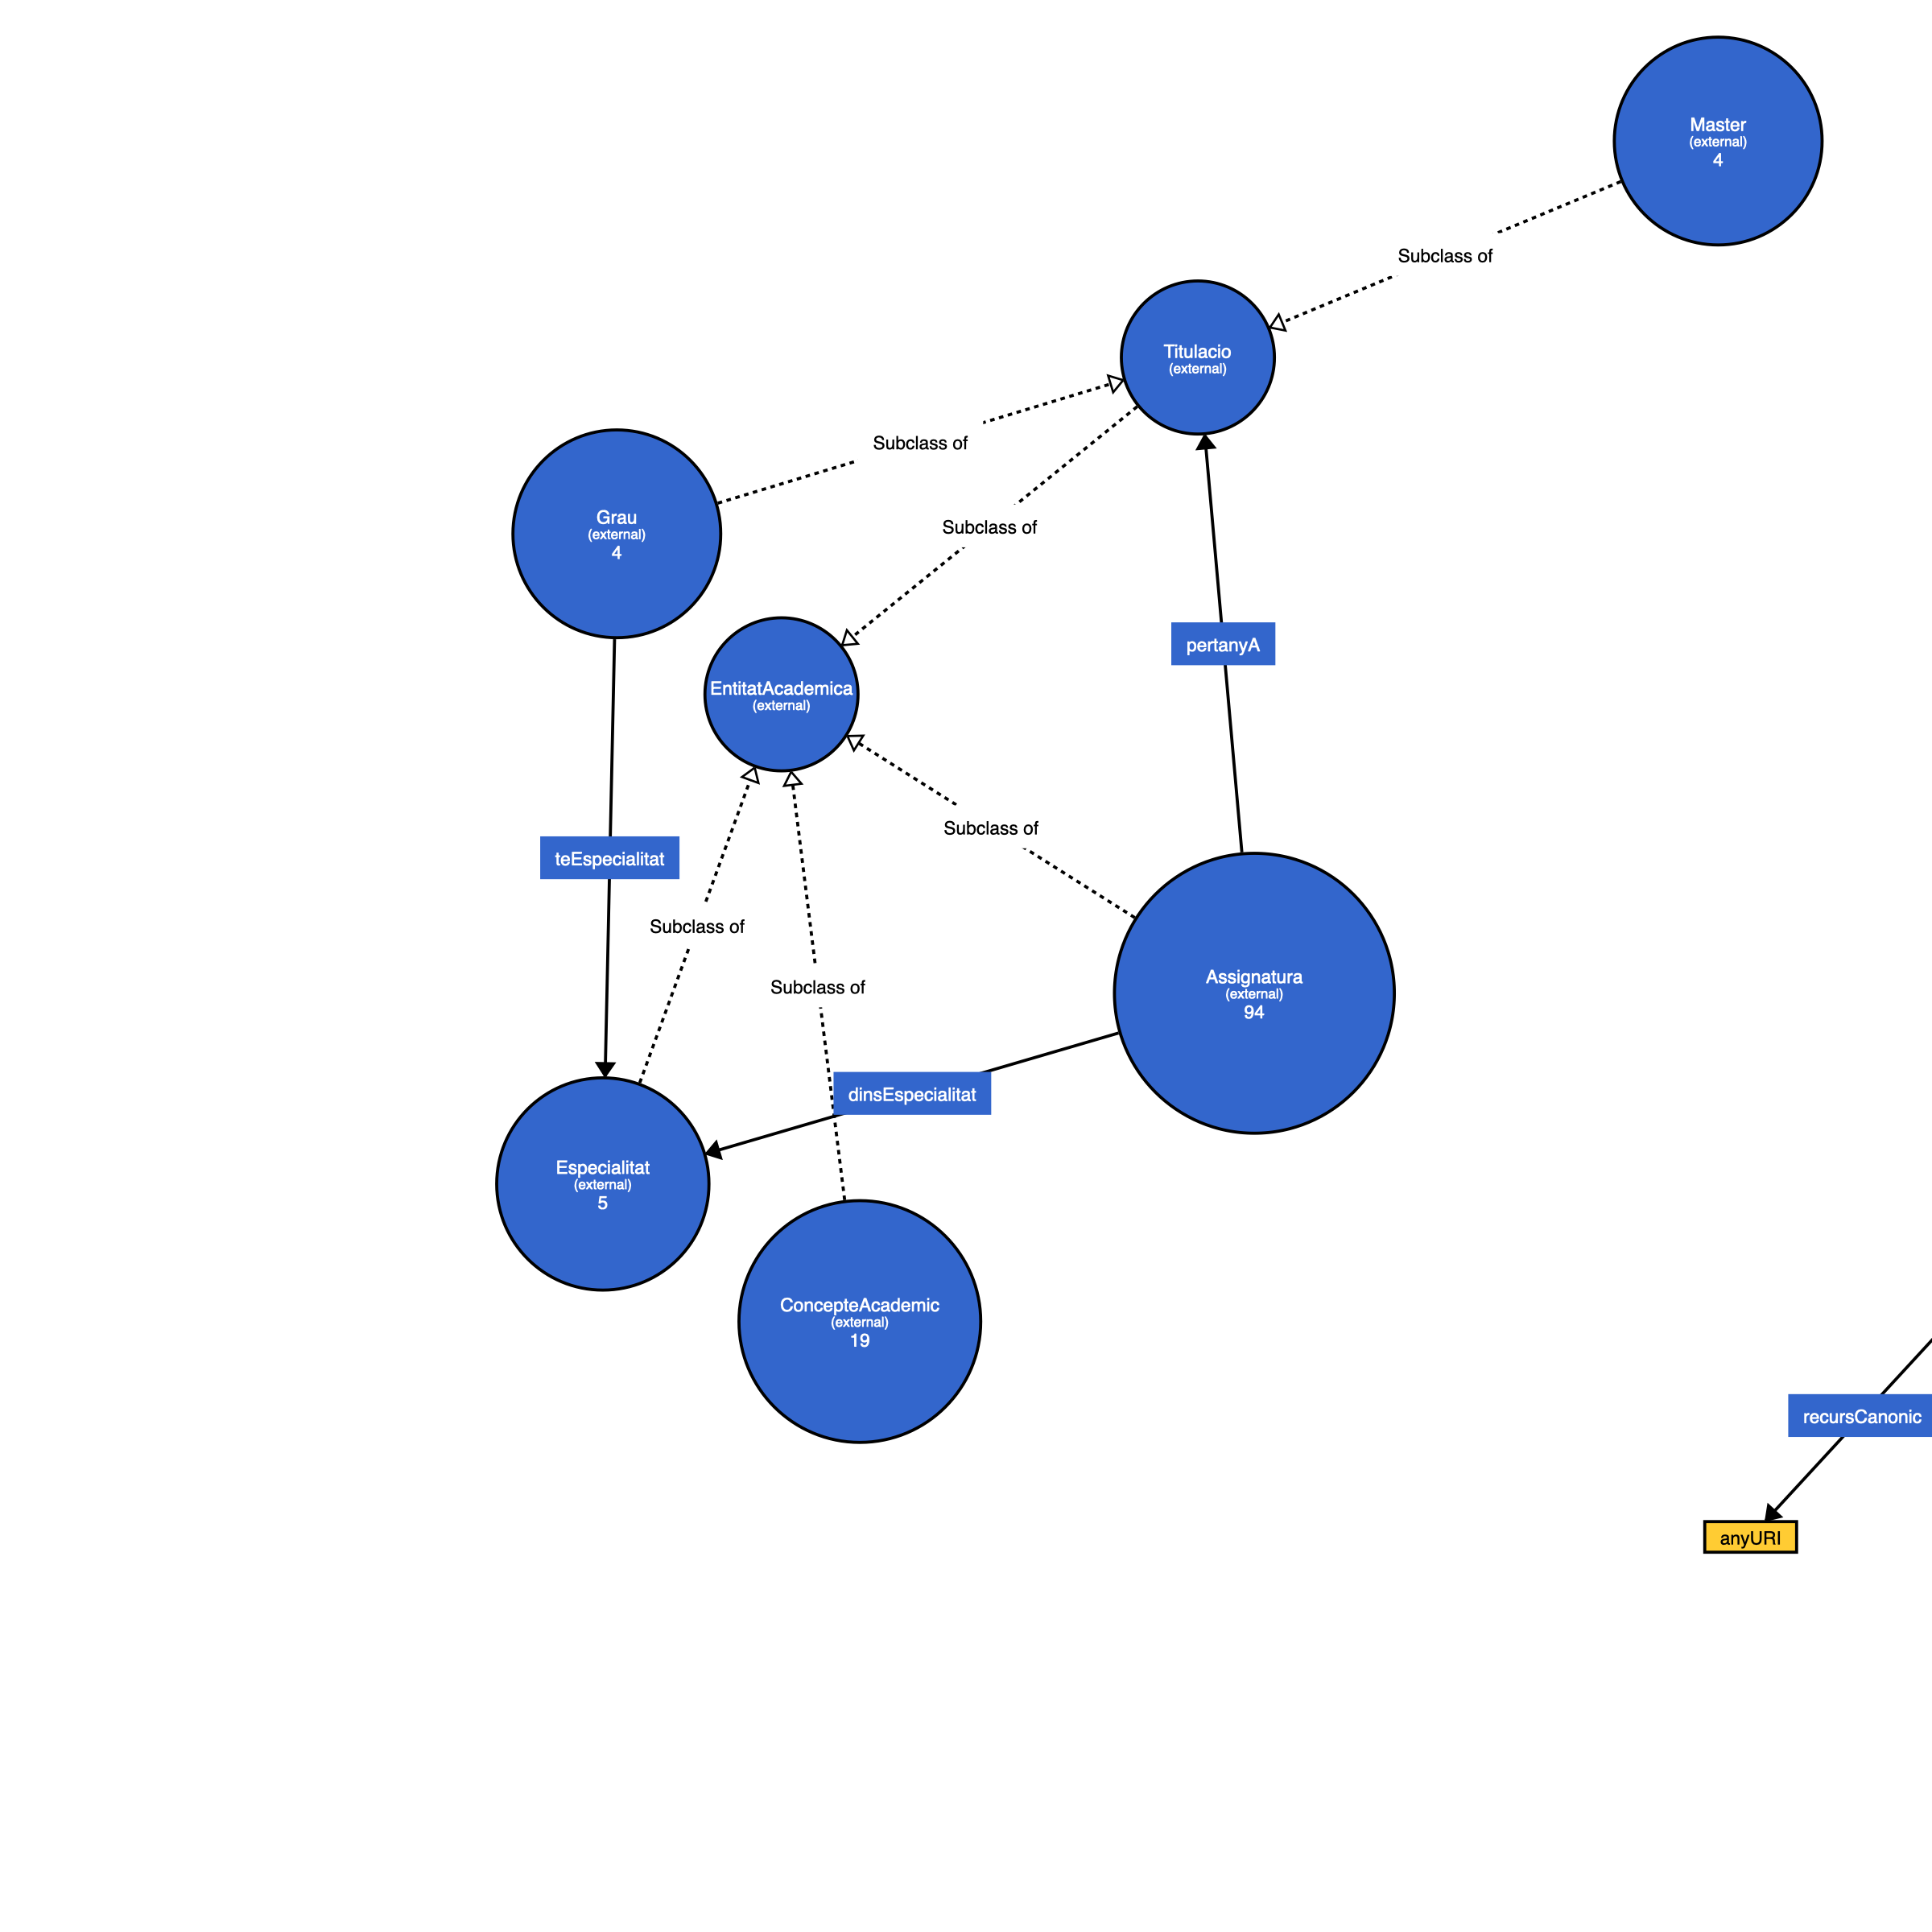
\includegraphics[width=\textwidth]{figures/fib_ontology_graph.png}
\caption{Visualizaci\'on del grafo RDF de la ontolog\'ia de la FIB. En el centro, las clases del esquema; alrededor, las instancias de asignaturas, titulaciones y conceptos con sus relaciones.}
\label{fig:ontology-graph}
\end{figure}

\subsection{API de consulta}

Sobre el grafo se construy\'o una capa de acceso (\texttt{fib\_ontology.py}) que carga el TTL en memoria y ofrece las operaciones que el resto del sistema necesita: detecci\'on de conceptos en una consulta (con normalizaci\'on de acentos y l\'imites de palabra), expansi\'on de t\'erminos v\'ia \texttt{skos:related}, recuperaci\'on de recursos can\'onicos y pesos, \'indices de c\'odigos de asignatura y siglas de titulaci\'on, y generaci\'on del contexto ontol\'ogico que se pasa al LLM. La expansi\'on usa SPARQL directamente sobre el grafo:

\begin{lstlisting}[language=SQL, caption={Consulta SPARQL de expansi\'on: t\'erminos relacionados de un concepto detectado}, label={lst:sparql_expansion}]
PREFIX skos: <http://www.w3.org/2004/02/skos/core#>
PREFIX fib:  <http://www.fib.upc.edu/ontology#>

SELECT ?relatedLabel ?canonicalUrl ?weight
WHERE {
  ?concept  skos:prefLabel  ?label ;
            skos:related    ?related .
  ?related  skos:prefLabel  ?relatedLabel ;
            fib:recursCanonic ?canonicalUrl ;
            fib:pesIntencio   ?weight .
}
\end{lstlisting}

Un ejemplo de ejecuci\'on completo, que adem\'as anticipa el mecanismo de re-ranqueo de la Secci\'on~\ref{sec:controlled}:

\begin{enumerate}
    \item \textbf{Consulta original:} \textit{``com m'apunto a les assignatures?''}
    \item \textbf{Detecci\'on:} ``m'apunto'' coincide con una \texttt{skos:altLabel} del concepto \texttt{Matr\'icula}.
    \item \textbf{Expansi\'on:} v\'ia \texttt{skos:related} se a\~naden ``places lliures'' y ``calendari acad\`emic''.
    \item \textbf{Recursos:} se recupera la URL can\'onica de matr\'icula y su \texttt{pesIntencio} (0.20).
    \item \textbf{Resultado:} la p\'agina oficial de matr\'icula entra garantizada en el \textit{pool} de candidatos y recibe un \textit{boost} en el re-ranqueo, aunque el fraseo informal del estudiante no comparta ni una palabra con el texto de la p\'agina.
\end{enumerate}

\section{Indexaci\'on: del HTML a ChromaDB}
\label{sec:ingesta}

La ingesta (\texttt{ingest.py}) transforma los documentos scrapeados en chunks indexados. Esta parte sufri\'o m\'as reescrituras de las que me gustar\'ia admitir, porque cada problema de calidad de datos que aparec\'ia aguas arriba acababa manifest\'andose como un fallo de recuperaci\'on aguas abajo, dif\'icil de diagnosticar.

\subsection{Deduplicaci\'on con prioridad can\'onica}
\label{sec:dedup}

El primer problema serio: al evaluar las primeras versiones, hab\'ia consultas que fallaban de forma aparentemente aleatoria. Investigando, descubr\'i que la causa estaba en la deduplicaci\'on. Muchas p\'aginas de la FIB tienen \textbf{contenido id\'entico bajo URLs distintas} (la misma p\'agina de plazas libres servida para varios grados). Mi deduplicaci\'on inicial, por hash de contenido, se quedaba con una URL \textit{arbitraria} de cada grupo de duplicados. El resultado: a veces la URL can\'onica que la ontolog\'ia esperaba no estaba indexada, y todo el mecanismo de inyecci\'on y boosts fallaba silenciosamente.

La soluci\'on fue hacer la deduplicaci\'on \textbf{consciente de la ontolog\'ia}: cuando varios documentos comparten contenido, se conserva como representante la versi\'on cuya URL es can\'onica seg\'un el grafo (\texttt{recursCanonic}), y el resto de URLs se guardan como metadato \texttt{duplicate\_urls}. Es un detalle peque\~no, pero ilustra bien una lecci\'on transversal del proyecto: \textbf{la ontolog\'ia solo es \'util si el \'indice y el grafo son coherentes entre s\'i}.

\subsection{Chunking sem\'antico}

La primera versi\'on troceaba el texto cada $N$ caracteres, cortando frases por la mitad; los embeddings de esos fragmentos eran sem\'anticamente confusos. La versi\'on final usa un divisor recursivo (\texttt{RecursiveCharacterTextSplitter}) que intenta cortar por p\'arrafos, luego por frases y solo en \'ultimo caso por palabras, con chunks de $\sim$1.000 caracteres y solapamiento de 150. Adem\'as, el texto que se vectoriza incluye el \textbf{t\'itulo de la p\'agina y la secci\'on} como prefijo, lo que da contexto al embedding (un chunk que dice ``el per\'iode s'obre al juliol'' es ambiguo; precedido de ``Matr\'icula > Per\'iodes'' deja de serlo).

\subsection{Filtrado de fragmentos de bajo valor y p\'aginas de aterrizaje}
\label{sec:filtering}

El scraping produce inevitablemente ruido: migas de pan, men\'us, avisos de cookies, fragmentos residuales de pocas palabras. Se a\~nadi\'o un filtro que descarta chunks de menos de \textbf{120 caracteres} (\texttt{MIN\_CHUNK\_LENGTH}) o con menos de un 50\% de contenido alfab\'etico.

Pero este filtro, tal cual, creaba un problema con las \textbf{p\'aginas de aterrizaje cr\'iticas}: horarios, ex\'amenes, profesorado o plazas libres tienen poqu\'isimo texto est\'atico (su contenido es din\'amico), y el filtro las eliminaba del \'indice\dots{} justo las p\'aginas que m\'as se consultan. La soluci\'on fue una regla de excepci\'on: \textbf{las p\'aginas cuya URL es un recurso can\'onico de la ontolog\'ia se indexan siempre}, con un umbral m\'inimo reducido (30 caracteres). De nuevo, la ontolog\'ia actuando como fuente de verdad sobre qu\'e es importante, independientemente del volumen de texto.

\subsection{Identificadores robustos e idempotencia}

Un \'ultimo problema de ingenier\'ia que vale la pena documentar porque cost\'o varias horas de depuraci\'on: los identificadores de chunk originales (URL + primeros 200 caracteres) colisionaban cuando dos chunks empezaban igual, y ChromaDB rechazaba \textbf{lotes enteros} de 32 chunks por una sola colisi\'on, perdiendo documentos de forma silenciosa. La versi\'on final usa IDs deterministas (hash de URL + \'indice de chunk + hash del texto) y operaciones \textit{upsert}, de modo que re-ejecutar la ingesta es idempotente y nunca pierde datos.

\section{Las cinco estrategias de recuperaci\'on}
\label{sec:estrategias}

Con el \'indice estable, el trabajo se centr\'o en la pregunta central del TFG: ?`c\'omo recuperar mejor? Para poder responderla con rigor, todas las estrategias se implementaron bajo una \textbf{interfaz com\'un} (\texttt{retrieval/base.py}): cada retriever recibe una consulta y devuelve una lista de resultados homog\'eneos (documento, metadatos, score, fuente de recuperaci\'on, boosts aplicados). Esto permite conmutarlas desde la UI y evaluarlas con el mismo script.

\subsection{Baseline 1: BM25 (l\'exico)}

El baseline l\'exico (\texttt{retrieval/bm25.py}) carga todos los chunks del \'indice, los tokeniza con normalizaci\'on de acentos y \textit{stopwords} de catal\'an y castellano, y construye un \'indice Okapi BM25 en memoria (Secci\'on~\ref{sec:bm25}). Su perfil es el esperado: excelente cuando la consulta comparte t\'erminos exactos con el documento (c\'odigos, nombres propios), in\'util ante sinonimia o cambios de idioma.

\subsection{Baseline 2: b\'usqueda vectorial pura (dense)}

El baseline vectorial (\texttt{retrieval/dense.py}) es el RAG cl\'asico: embedding de la consulta con MiniLM y b\'usqueda por similitud coseno en ChromaDB. Era el comportamiento de la primera versi\'on del sistema completo, y conviene subrayarlo: \textbf{todo lo que viene despu\'es se mide contra esto}.

\subsection{Estrategia 3: expansi\'on ontol\'ogica naive}
\label{sec:ontology-naive}

La primera idea ``sem\'antica'' fue la m\'as intuitiva: detectar conceptos de la ontolog\'ia en la consulta y a\~nadir sus t\'erminos relacionados antes de la b\'usqueda vectorial (\texttt{retrieval/ontology\_expansion.py}). Por ejemplo, \textit{``quan puc matricular-me?''} se convierte en \textit{``quan puc matricular-me? matr\'icula places lliures calendari acad\`emic''}.

Mi expectativa era que esto mejorar\'ia claramente al baseline. El resultado real (anticipo de la Tabla~\ref{tab:retrieval-metrics}): mejora marginal, casi ruido. El an\'alisis de errores fue revelador: a\~nadir t\'erminos al texto de la consulta \textbf{diluye el embedding} ---el vector resultante es un promedio sem\'antico de m\'as cosas--- y solo ayuda cuando la consulta original era demasiado escueta. Este resultado negativo fue el punto de inflexi\'on del proyecto: la ontolog\'ia no aporta valor \textit{reescribiendo la consulta}, sino \textit{decidiendo qu\'e documentos importan}. Eso es exactamente lo que hace la estrategia siguiente.

\subsection{Vinculaci\'on de entidades (Entity Linking)}
\label{sec:entity-linking}

Antes de la estrategia controlada hay que explicar su pieza m\'as delicada. Durante el an\'alisis de errores apareci\'o un patr\'on recurrente: las consultas con \textbf{siglas o c\'odigos} (\textit{``temari de XC''}, \textit{``qu\`e necessito per fer el TFG?''}, \textit{``notes de tall del GEI''}) fallaban estrepitosamente en los dos baselines. Para BM25, ``XC'' es un token rar\'isimo que adem\'as aparece poco en la p\'agina de la propia asignatura; para el embedding, una sigla de dos letras apenas aporta se\~nal sem\'antica.

La soluci\'on (\texttt{retrieval/entity\_linker.py}) explota los \'indices de c\'odigos de la ontolog\'ia: las $\sim$94 asignaturas con su \texttt{codi} y las titulaciones con sus siglas. La detecci\'on usa expresiones regulares con \textbf{l\'imites de palabra} (\verb|\b|) sobre la consulta, con reglas de sensibilidad a may\'usculas que tuvieron que refinarse emp\'iricamente:

\begin{itemize}
  \item Los c\'odigos en general se detectan \textit{case-insensitive}, porque los estudiantes escriben ``xc'' o ``prop'' sin may\'usculas.
  \item Sin embargo, hay c\'odigos que colisionan con palabras comunes del catal\'an/castellano: \texttt{CAP}, \texttt{PES}, \texttt{PAR}, \texttt{MAI}, \texttt{BIO}, \texttt{SOA}, \texttt{IES}, \texttt{EDO}, \texttt{ROB}. La consulta \textit{``quina nota cal per entrar?''} no menciona la asignatura CAP, aunque contenga la palabra ``cap''. Para este conjunto de \textbf{c\'odigos ambiguos}, el emparejamiento exige may\'usculas exactas: ``CAP'' s\'i dispara la vinculaci\'on, ``cap'' no.
\end{itemize}

Esta lista de c\'odigos ambiguos se construy\'o mediante an\'alisis de falsos positivos sobre las consultas de desarrollo, y es un buen ejemplo del tipo de conocimiento de dominio ---peque\~no, aburrido, decisivo--- que no aparece en ning\'un paper pero marca la diferencia entre un sistema que funciona y uno que no.

Cada entidad vinculada se resuelve a su \textbf{URL can\'onica} v\'ia el grafo, y esa informaci\'on se entrega al re-ranqueador.

\subsection{Estrategia 4: b\'usqueda controlada por ontolog\'ia}
\label{sec:controlled}

La estrategia principal del trabajo (\texttt{retrieval/controlled\_ontology.py}) reorganiza el papel de la ontolog\'ia seg\'un la lecci\'on de la Secci\'on~\ref{sec:ontology-naive}: en lugar de modificar la consulta, \textbf{controla el conjunto de candidatos y su orden}. El algoritmo tiene cuatro fases:

\begin{enumerate}
  \item \textbf{Recuperaci\'on amplia.} Se recuperan hasta $\max(8k, 40)$ candidatos de ChromaDB, usando tanto la consulta original como la enriquecida. La idea es que el recall bruto deje de ser el cuello de botella: el trabajo fino se hace despu\'es, en el re-ranqueo.
  \item \textbf{Inyecci\'on de p\'aginas can\'onicas.} Para cada entidad vinculada y cada concepto detectado, se buscan en el \'indice los chunks de su URL can\'onica y se \textbf{inyectan} en el pool de candidatos si no estaban. Esto garantiza que la p\'agina oficial de XC est\'a en el pool cuando alguien pregunta por XC, tenga la similitud que tenga.
  \item \textbf{Score base honesto.} Los documentos inyectados necesitan un score comparable al de los recuperados. Mi primera implementaci\'on les asignaba un valor fijo, pero esto distorsionaba el ranking de formas dif\'iciles de razonar (a veces demasiado alto, a veces insuficiente). La versi\'on final calcula la \textbf{similitud coseno real} entre el embedding de la consulta y el embedding almacenado de cada chunk inyectado: as\'i todos los candidatos compiten en la misma escala y los boosts posteriores tienen una sem\'antica clara (``cu\'anto conf\'io en la se\~nal ontol\'ogica por encima de la sem\'antica'').
  \item \textbf{Re-ranqueo guiado por el grafo.} Sobre el score base se aplican boosts aditivos cuyos valores y patrones \textbf{provienen de la ontolog\'ia}, no de reglas codificadas:
  \begin{itemize}
    \item \textbf{Entidad vinculada} ($+0.45$): el chunk pertenece a la URL can\'onica de una entidad detectada en la consulta. Es el boost m\'as alto porque la se\~nal es casi inequ\'ivoca.
    \item \textbf{Concepto detectado} ($+\,\texttt{pesIntencio}$): el chunk pertenece a la URL can\'onica de un concepto detectado; la magnitud la decide el grafo (entre 0.12 y 0.30 seg\'un la especificidad del concepto).
    \item \textbf{Coincidencia de slug} ($+\,\texttt{pesIntencio} \times 0.5$): la URL del chunk contiene el \texttt{patroUrl} del concepto sin ser la p\'agina can\'onica (p\'aginas hijas).
    \item \textbf{\'Ambito de titulaci\'on} ($+0.15$): si la consulta menciona una titulaci\'on (``del GEI''), los chunks de su sub\'arbol de URLs reciben un impulso, lo que desambigua entre las p\'aginas equivalentes de grados distintos.
  \end{itemize}
\end{enumerate}

Quiero subrayar la diferencia entre esto y un sistema de reglas \textit{hardcodeadas}: aqu\'i el c\'odigo solo define los \textit{mecanismos} (inyecci\'on, tipos de boost), mientras que el \textit{conocimiento} (qu\'e URL es can\'onica de qu\'e, con qu\'e peso, con qu\'e patrones) vive en el grafo RDF y se consulta en tiempo de ejecuci\'on. A\~nadir un concepto nuevo no requiere tocar el c\'odigo: basta a\~nadirlo a la ontolog\'ia y reconstruir el TTL (requisito RNF05).

\subsection{Estrategia 5: fusi\'on h\'ibrida (RRF)}
\label{sec:hybrid-impl}

La \'ultima estrategia (\texttt{retrieval/hybrid\_rrf.py}) fusiona los rankings de dense, BM25 y controlada mediante \textit{Reciprocal Rank Fusion} (Secci\'on~\ref{sec:rrf}), con $k=60$ y pesos $1.0/0.6/0.6$ (controlada/BM25/dense). La fusi\'on se hace a nivel de URL ---no de chunk--- para que varios fragmentos de la misma p\'agina no compitan entre s\'i.

La motivaci\'on te\'orica es s\'olida (se\~nales complementarias), y de hecho la literatura suele recomendar h\'ibridos por defecto. Como se ver\'a en la evaluaci\'on, en nuestro dominio el resultado fue otro, y entender por qu\'e es uno de los an\'alisis m\'as interesantes del Cap\'itulo~\ref{ch:evaluacion}.

\section{Pipeline RAG y generaci\'on}

\subsection{Condensaci\'on de preguntas de seguimiento}

Un problema cl\'asico de los chatbots RAG que apareci\'o en cuanto empec\'e a probar conversaciones reales: la segunda pregunta del usuario (\textit{``i quan obre el per\'iode?''}) es irresoluble sin el contexto de la primera (\textit{``com funciona la matr\'icula?''}). La soluci\'on est\'andar, que adopt\'e, es la \textbf{condensaci\'on}: antes de recuperar, un LLM reescribe la pregunta de seguimiento como pregunta aut\'onoma usando el historial (\textit{``quan obre el per\'iode de matr\'icula?''}), y es esa pregunta condensada la que entra al retriever. El coste es una llamada extra al LLM solo cuando hay historial.

\subsection{Prompt y fundamentaci\'on}

El prompt del sistema instruye al modelo para responder \textbf{exclusivamente} con la informaci\'on de los documentos recuperados, en el idioma del usuario, citando las fuentes, y declarando expl\'icitamente cuando la informaci\'on no est\'a disponible. Adem\'as de los documentos, el prompt incluye el \textbf{contexto ontol\'ogico}: los conceptos detectados, sus relaciones y sus recursos can\'onicos, en formato estructurado. En las pruebas cualitativas esto redujo visiblemente las respuestas evasivas en preguntas sobre entidades (el modelo ``sabe'' que XC es Xarxes de Computadors y pertenece al GEI aunque el chunk recuperado no lo diga).

\section{Interfaz de usuario}

La interfaz (\texttt{app.py}, Streamlit) evolucion\'o de un chat simple a una herramienta de demostraci\'on y an\'alisis del sistema completo:

\begin{itemize}
  \item \textbf{Chat conversacional} con historial, fuentes citadas y streaming de la respuesta.
  \item \textbf{Selector de estrategia} en la barra lateral: las cinco estrategias son conmutables en vivo, lo que convierte la UI en una demo directa del experimento central del TFG.
  \item \textbf{Detalles t\'ecnicos por respuesta}: un panel expandible muestra el flujo completo de la consulta (original $\rightarrow$ condensada $\rightarrow$ enriquecida), las entidades vinculadas, y cada documento recuperado con su score, similitud y los boosts aplicados como etiquetas.
  \item \textbf{Explorador de la ontolog\'ia}: permite navegar el grafo por clase e instancia, viendo etiquetas SKOS, relaciones, recursos can\'onicos y pesos. Cumple una funci\'on did\'actica: hacer visible el conocimiento que gu\'ia la b\'usqueda.
  \item \textbf{Comparador de estrategias}: dada una consulta, la ejecuta contra los cinco modos en paralelo y muestra el top-3 de URLs de cada uno en una tabla. Fue una herramienta de an\'alisis de errores durante el desarrollo que acab\'o integrada en la UI.
\end{itemize}

Los componentes pesados (\'indice vectorial, grafo de la ontolog\'ia, cadena RAG) se cachean como recursos de Streamlit, de modo que el cambio de estrategia es instant\'aneo y la \'unica latencia perceptible es la generaci\'on del LLM.

% ============================================================================
\chapter{Evaluaci\'on y Resultados}
\label{ch:evaluacion}
% ============================================================================

\section{Dise\~no de la evaluaci\'on}

\subsection{Del an\'alisis cualitativo a la evaluaci\'on formal}

La primera versi\'on del sistema se ``evaluaba'' de manera informal: probaba consultas a mano y miraba si la respuesta parec\'ia razonable. Esto sirve para desarrollar, pero no para sostener ninguna afirmaci\'on de la memoria. La evaluaci\'on definitiva se dise\~n\'o con tres principios:

\begin{enumerate}
  \item \textbf{Autom\'atica y reproducible:} un script (\texttt{evaluation/evaluate.py}) ejecuta todas las estrategias contra el mismo banco de consultas y produce los resultados en CSV/JSON con marca de tiempo. Cualquier cifra de este cap\'itulo se puede regenerar con un comando.
  \item \textbf{Centrada en la recuperaci\'on:} se eval\'ua qu\'e documentos devuelve cada estrategia, no el texto generado por el LLM. La raz\'on es metodol\'ogica: la generaci\'on es id\'entica en todos los modos, de manera que cualquier diferencia de calidad proviene de la recuperaci\'on; y evaluar texto generado requerir\'ia jueces humanos o LLM-as-judge, con la variabilidad que conllevan.
  \item \textbf{Con control del sobreajuste:} las reglas y el vocabulario de la ontolog\'ia se refinaron mediante an\'alisis de errores, y eso crea un riesgo real de ajustarse al banco de pruebas. La mitigaci\'on se explica a continuaci\'on.
\end{enumerate}

\subsection{El banco de consultas (golden set)}
\label{sec:golden-set}

Se construy\'o un conjunto de \textbf{40 consultas} (\texttt{evaluation/queries.json}) representativas de lo que pregunta un estudiante real: matr\'icula y tr\'amites, asignaturas por c\'odigo y por nombre, notas de corte, horarios y ex\'amenes, becas, movilidad, pr\'acticas, TFG, servicios\dots{} Las consultas est\'an escritas en catal\'an y castellano, con fraseos coloquiales (\textit{``com m'apunto a les assignatures?''}) adem\'as de formales, porque el desalineamiento de vocabulario es precisamente el fen\'omeno que queremos medir. Cada consulta tiene anotadas sus \textbf{URLs relevantes}, verificadas manualmente contra la web de la FIB.

La decisi\'on m\'as importante del dise\~no es la \textbf{divisi\'on dev/test}: 20 consultas de desarrollo (\textit{dev}) que s\'i utilic\'e para analizar errores y refinar el vocabulario de la ontolog\'ia, y \textbf{20 consultas de test (held-out) que no se miraron durante el desarrollo}. La comparaci\'on entre ambos conjuntos permite detectar sobreajuste: si una estrategia funciona en dev pero se hunde en test, sus reglas est\'an memorizando el banco de pruebas en lugar de generalizar. Esta precauci\'on result\'o muy informativa, como se ver\'a.

\subsection{M\'etricas}

Se emplean las m\'etricas est\'andar de recuperaci\'on de informaci\'on, calculadas sobre las URLs \'unicas del top-5 de cada estrategia:

\begin{itemize}
  \item \textbf{Hit@k} ($k = 1, 3, 5$): proporci\'on de consultas con al menos una URL relevante en el top-$k$. Hit@1 mide precisi\'on estricta; Hit@5, cobertura pr\'actica (en la UI se muestran 5 fuentes).
  \item \textbf{MRR} (\textit{Mean Reciprocal Rank}): media de $1/\text{rank}$ de la primera URL relevante. Premia que lo correcto est\'e arriba.
  \begin{equation}
    \text{MRR} = \frac{1}{|Q|} \sum_{i=1}^{|Q|} \frac{1}{\text{rank}_i}
  \end{equation}
  \item \textbf{P@5 / R@5}: precisi\'on y exhaustividad cl\'asicas en el top-5.
  \item \textbf{nDCG@5}: ganancia acumulada descontada normalizada, que pondera la relevancia por la posici\'on con descuento logar\'itmico.
\end{itemize}

\section{Resultados de la recuperaci\'on}
\label{sec:resultados-retrieval}

La Tabla~\ref{tab:retrieval-metrics} resume los resultados globales de las cinco estrategias sobre las 40 consultas.

\begin{table}[H]
\centering
\caption{Resultados globales de las cinco estrategias de recuperaci\'on (40 consultas)}
\label{tab:retrieval-metrics}
\begin{tabular}{lccccc}
\toprule
\textbf{Estrategia} & \textbf{Hit@1} & \textbf{Hit@3} & \textbf{Hit@5} & \textbf{MRR} & \textbf{nDCG@5} \\
\midrule
BM25 (l\'exico)            & 20,0\% & 47,5\% & 55,0\% & 0,337 & 0,347 \\
Dense (vectorial)          & 15,0\% & 30,0\% & 37,5\% & 0,233 & 0,245 \\
Expansi\'on ontol\'ogica   & 10,0\% & 30,0\% & 47,5\% & 0,234 & 0,264 \\
\textbf{Controlada (ontolog\'ia)} & \textbf{75,0\%} & \textbf{87,5\%} & \textbf{92,5\%} & \textbf{0,820} & \textbf{0,813} \\
H\'ibrida (RRF)            & 42,5\% & 62,5\% & 70,0\% & 0,525 & 0,532 \\
\bottomrule
\end{tabular}
\end{table}

\begin{figure}[H]
\centering
\begin{tikzpicture}
  \begin{scope}[yscale=0.06, xscale=2.2]
    % Axis
    \draw[-{Stealth[length=2mm]}] (0,0) -- (5.3,0);
    \draw[-{Stealth[length=2mm]}] (0,0) -- (0,105) node[above, font=\small] {\%};
    \foreach \y in {0,25,50,75,100} {
      \draw[gray!40] (0,\y) -- (5.2,\y);
      \node[left, font=\scriptsize] at (0,\y) {\y};
    }
    % Bars: Hit@1 (darker) and Hit@5 (lighter) per mode
    % BM25
    \fill[upcblue] (0.25,0) rectangle (0.45,20);
    \fill[fibblue!50] (0.50,0) rectangle (0.70,55);
    \node[below, font=\scriptsize, align=center] at (0.5,-2) {BM25};
    % Dense
    \fill[upcblue] (1.25,0) rectangle (1.45,15);
    \fill[fibblue!50] (1.50,0) rectangle (1.70,37.5);
    \node[below, font=\scriptsize, align=center] at (1.5,-2) {Dense};
    % Ontology expansion
    \fill[upcblue] (2.25,0) rectangle (2.45,10);
    \fill[fibblue!50] (2.50,0) rectangle (2.70,47.5);
    \node[below, font=\scriptsize, align=center] at (2.5,-2) {Expansi\'on};
    % Controlled
    \fill[upcblue] (3.25,0) rectangle (3.45,75);
    \fill[fibblue!50] (3.50,0) rectangle (3.70,92.5);
    \node[below, font=\scriptsize, align=center] at (3.5,-2) {Controlada};
    % Hybrid
    \fill[upcblue] (4.25,0) rectangle (4.45,42.5);
    \fill[fibblue!50] (4.50,0) rectangle (4.70,70);
    \node[below, font=\scriptsize, align=center] at (4.5,-2) {H\'ibrida};
    % Legend
    \fill[upcblue] (0.3,112) rectangle (0.5,118);
    \node[right, font=\scriptsize] at (0.55,115) {Hit@1};
    \fill[fibblue!50] (1.5,112) rectangle (1.7,118);
    \node[right, font=\scriptsize] at (1.75,115) {Hit@5};
  \end{scope}
\end{tikzpicture}
\caption{Hit@1 y Hit@5 de las cinco estrategias sobre el conjunto completo de 40 consultas.}
\label{fig:results-bars}
\end{figure}

Los resultados responden directamente a las tres preguntas de investigaci\'on del Cap\'itulo~\ref{ch:introduccion}:

\paragraph{P1 --- ?`Sirve la expansi\'on de consulta por s\'i sola?} Apenas. La expansi\'on ontol\'ogica naive mejora ligeramente el Hit@5 del baseline vectorial (47,5\% vs.\ 37,5\%) pero \textit{empeora} su Hit@1 (10\% vs.\ 15\%): los t\'erminos a\~nadidos amplifican el recall a costa de diluir la precisi\'on del embedding. Es un resultado negativo, coherente con la experiencia hist\'orica de la expansi\'on de consultas en IR \cite{bhogal2007review}, y para m\'i fue la lecci\'on m\'as formativa del proyecto.

\paragraph{P2 --- ?`Qu\'e aporta la integraci\'on profunda?} La diferencia entre usar la ontolog\'ia como diccionario (expansi\'on) y usarla como \textbf{fuente de conocimiento can\'onico} (estrategia controlada) es dr\'astica: de 47,5\% a \textbf{92,5\% de Hit@5}, y un MRR que pasa de 0,23 a \textbf{0,82}. La estrategia controlada multiplica por 2,5 el Hit@5 del mejor baseline y por 3,5 su Hit@1. El an\'alisis por categor\'ias muestra que la mejora se concentra exactamente donde se dise\~n\'o: consultas con siglas y c\'odigos (donde el entity linking inyecta la p\'agina correcta) y consultas sobre p\'aginas de aterrizaje de poco texto (donde la inyecci\'on can\'onica compensa la falta de se\~nal sem\'antica).

\paragraph{P3 --- ?`H\'ibrido o estrategia dominante?} Contra mi intuici\'on inicial, el h\'ibrido RRF (70\% Hit@5) qued\'o claramente por debajo de la estrategia controlada sola. La Secci\'on~\ref{sec:eval-hybrid} analiza el porqu\'e.

\subsection{Generalizaci\'on: dev vs.\ test}
\label{sec:dev-test}

La Tabla~\ref{tab:dev-test} desglosa los resultados por partici\'on, que es donde se comprueba si las reglas generalizan o memorizan.

\begin{table}[H]
\centering
\caption{Desglose por partici\'on: 20 consultas de desarrollo vs.\ 20 consultas held-out}
\label{tab:dev-test}
\begin{tabular}{llcccc}
\toprule
\textbf{Estrategia} & \textbf{Split} & \textbf{Hit@1} & \textbf{Hit@5} & \textbf{MRR} & \textbf{nDCG@5} \\
\midrule
\multirow{2}{*}{BM25}       & dev  & 20,0\% & 70,0\% & 0,406 & 0,461 \\
                            & test & 20,0\% & 40,0\% & 0,268 & 0,233 \\
\midrule
\multirow{2}{*}{Dense}      & dev  & 10,0\% & 35,0\% & 0,189 & 0,229 \\
                            & test & 20,0\% & 40,0\% & 0,277 & 0,261 \\
\midrule
\multirow{2}{*}{Expansi\'on} & dev  & 10,0\% & 45,0\% & 0,238 & 0,284 \\
                            & test & 10,0\% & 50,0\% & 0,231 & 0,244 \\
\midrule
\multirow{2}{*}{\textbf{Controlada}} & dev  & \textbf{80,0\%} & \textbf{95,0\%} & \textbf{0,867} & \textbf{0,869} \\
                            & test & \textbf{70,0\%} & \textbf{90,0\%} & \textbf{0,773} & \textbf{0,758} \\
\midrule
\multirow{2}{*}{H\'ibrida}  & dev  & 50,0\% & 75,0\% & 0,602 & 0,626 \\
                            & test & 35,0\% & 65,0\% & 0,448 & 0,438 \\
\bottomrule
\end{tabular}
\end{table}

La lectura clave: la estrategia controlada cae solo 5 puntos de Hit@5 entre dev y test (95\% $\rightarrow$ 90\%), una degradaci\'on moderada que indica que \textbf{los mecanismos generalizan} a consultas no vistas. El conocimiento que explota (URLs can\'onicas, c\'odigos, relaciones) es estructural del dominio, no espec\'ifico de las consultas con las que se desarroll\'o. En contraste, BM25 se desploma de 70\% a 40\%: su buen resultado en dev depend\'ia de coincidencias l\'exicas afortunadas que no se repiten en test.

Esta tabla es tambi\'en una declaraci\'on metodol\'ogica: habr\'ia sido f\'acil reportar solo los resultados de dev (95\% de Hit@5 queda mejor que 92,5\%), pero el valor de la evaluaci\'on est\'a precisamente en demostrar que el sistema no est\'a sobreajustado.

\section{Impacto de la ontolog\'ia: an\'alisis por mecanismo}
\label{sec:impacto-ontologia}

Dado que la estrategia controlada combina varios mecanismos, conviene atribuir la mejora. Del an\'alisis de los resultados detallados (fichero \texttt{details} de la evaluaci\'on) se extraen tres patrones:

\begin{enumerate}
  \item \textbf{El entity linking es decisivo en las consultas sobre asignaturas} (5 de las 40, adem\'as de las que mencionan siglas de titulaci\'on). En dense, este tipo de consulta falla casi siempre (la sigla no aporta se\~nal); con vinculaci\'on + inyecci\'on, la p\'agina de la asignatura aparece en el top-1 de manera consistente.
  \item \textbf{La inyecci\'on can\'onica rescata las p\'aginas de aterrizaje.} Horarios, ex\'amenes, plazas libres: p\'aginas casi sin texto que ninguna estrategia de contenido puede encontrar. La combinaci\'on indexaci\'on-forzada (Secci\'on~\ref{sec:filtering}) + inyecci\'on + boost las pone arriba cuando el concepto se detecta.
  \item \textbf{El \'ambito de titulaci\'on resuelve la ambig\"uedad entre grados.} Consultas como ``places lliures del GEI'' devolv\'ian antes la p\'agina equivalente de otro grado (contenido casi id\'entico); el boost de sub\'arbol corrige la mayor\'ia de estos casos.
\end{enumerate}

Igual de informativo es lo que \textbf{no} funcion\'o: la expansi\'on de t\'erminos, que era mi apuesta inicial, result\'o ser el mecanismo menos valioso. Si tuviera que resumir el hallazgo central del TFG en una frase: \textit{en un dominio cerrado, la ontolog\'ia aporta m\'as como mapa de recursos can\'onicos que como diccionario de sin\'onimos}.

\section{Evaluaci\'on de la estrategia h\'ibrida (RRF)}
\label{sec:eval-hybrid}

El resultado del h\'ibrido merece secci\'on propia porque contradice la recomendaci\'on habitual de la literatura (``cuando dudes, fusiona''). Con 70\% de Hit@5 y MRR 0,525, el RRF qued\'o 22,5 puntos por debajo de la estrategia controlada que es uno de sus componentes. ?`C\'omo puede una fusi\'on empeorar a su mejor miembro?

La explicaci\'on est\'a en la aritm\'etica del RRF. La fusi\'on por rango asume que los sistemas combinados tienen \textbf{calidades comparables}; cuando uno es claramente superior (controlada: 0,82 MRR) y los otros notablemente inferiores (BM25: 0,34; dense: 0,23), cada documento irrelevante que BM25 o dense colocan en sus primeras posiciones recibe una puntuaci\'on RRF alta y \textbf{desplaza hacia abajo los documentos correctos} de la estrategia controlada. El ruido de los d\'ebiles diluye la precisi\'on del fuerte: en consultas de matr\'icula o calendario, BM25 aporta documentos lexicalmente relacionados (menciones de ``matr\'icula'' en noticias, normativas antiguas) que no son las p\'aginas can\'onicas.

Lo intent\'e mitigar bajando los pesos de los componentes d\'ebiles ($1.0/0.6/0.6$), lo que mejor\'o algo el resultado, pero la conclusi\'on emp\'irica se mantiene: \textbf{en este dominio, la fusi\'on solo tendr\'ia sentido si los componentes fueran m\'as equilibrados}. Decid\'i documentar el resultado negativo en lugar de esconderlo, porque responde limpiamente a P3 y porque el an\'alisis del fallo (diluci\'on por desequilibrio de calidad) es generalizable a otros sistemas RAG.

Una reflexi\'on adicional: la estrategia controlada ya es, internamente, un h\'ibrido ---combina similitud sem\'antica con conocimiento estructurado--- pero con una integraci\'on \textit{jer\'arquica} (la sem\'antica propone, la ontolog\'ia corrige) en lugar de \textit{democr\'atica} (todos votan). Los resultados sugieren que en dominios cerrados con conocimiento curado, la integraci\'on jer\'arquica es preferible.

\section{Evaluaci\'on cualitativa del sistema completo}

Adem\'as de las m\'etricas de recuperaci\'on, se realizaron pruebas cualitativas del pipeline completo (recuperaci\'on + generaci\'on) con conversaciones reales. Algunas observaciones:

\begin{itemize}
  \item Las respuestas generadas son fieles a los documentos: el prompt restrictivo y el contexto ontol\'ogico hacen que el modelo decline responder cuando no tiene la informaci\'on, en lugar de inventar.
  \item La condensaci\'on de preguntas funciona bien en seguimientos directos (``i quan obre?'') y razonablemente en cambios de tema parciales.
  \item La latencia de generaci\'on con Llama 3.2 (3B) en CPU es perceptible (varios segundos hasta el primer token), aunque la recuperaci\'on en s\'i se mantiene por debajo de los 2 segundos del requisito RNF01.
\end{itemize}

\section{Evaluaci\'on con usuarios (SUS): dise\~no del estudio}
\label{sec:sus}

% NOTA IMPORTANTE: esta seccion describe el DISENO del estudio de usabilidad.
% La tabla de resultados esta comentada y debe rellenarse UNICAMENTE con datos
% reales una vez realizado el test con participantes. No incluir datos inventados.

Para complementar la evaluaci\'on cuantitativa de la recuperaci\'on con una medida de la experiencia de uso, se ha dise\~nado un estudio de usabilidad basado en el \textbf{System Usability Scale} (SUS) \cite{brooke1996}, el cuestionario est\'andar de 10 \'items con escala Likert de 5 puntos, cuya puntuaci\'on agregada (0--100) permite situar el sistema en percentiles bien estudiados (la media de la industria se sit\'ua en 68; por encima de 80 se considera excelente).

\subsection{Metodolog\'ia dise\~nada}

\begin{itemize}
  \item \textbf{Participantes:} 4--6 estudiantes de grado de la FIB, usuarios habituales de la web de la facultad, sin relaci\'on con el proyecto.
  \item \textbf{Tareas:} cada participante resuelve 4 tareas representativas usando \'unicamente SemanticFIB: (1) averiguar el per\'iodo de matr\'icula, (2) encontrar el temario de una asignatura concreta (p.ej.\ Xarxes de Computadors), (3) consultar el calendario de ex\'amenes, (4) comprobar las plazas libres de su grado.
  \item \textbf{Protocolo:} sin ayuda del facilitador; se registra si la tarea se completa y el tiempo aproximado. Al finalizar, el participante rellena el cuestionario SUS y se recoge feedback libre.
  \item \textbf{An\'alisis:} puntuaci\'on SUS individual y media, tasa de \'exito por tarea, y s\'intesis del feedback cualitativo.
\end{itemize}

% --- PLANTILLA DE RESULTADOS (descomentar y rellenar con datos reales) ---
% \begin{table}[H]
% \centering
% \caption{Resultados del cuestionario SUS}
% \label{tab:sus-results}
% \begin{tabular}{lcc}
% \toprule
% \textbf{Participante} & \textbf{Perfil} & \textbf{Puntuaci\'on SUS} \\
% \midrule
% P1 & Estudiante GEI (Qx) & -- \\
% P2 & Estudiante GEI (Qx) & -- \\
% P3 & Estudiante GEI (Qx) & -- \\
% P4 & Estudiante GEI (Qx) & -- \\
% \midrule
% \multicolumn{2}{r}{\textbf{Media}} & \textbf{--} \\
% \bottomrule
% \end{tabular}
% \end{table}

En el momento de redactar esta memoria el estudio est\'a dise\~nado y pendiente de ejecuci\'on con participantes reales; los resultados se incorporar\'an en la versi\'on final del documento. Las pruebas informales realizadas durante el desarrollo con compa\~neros apuntan a dos l\'ineas de mejora ya identificadas: la latencia del primer token cuando el LLM se ejecuta en CPU, y la conveniencia de poder exportar la conversaci\'on.

\section{Limitaciones observadas}
\label{sec:limitaciones}

Un an\'alisis honesto de los resultados debe incluir lo que el sistema no hace bien:

\begin{enumerate}
  \item \textbf{Dependencia de la cobertura de la ontolog\'ia.} La estrategia controlada solo despliega su ventaja cuando detecta algo (concepto, entidad, titulaci\'on). En las consultas de test que fallaron, la causa dominante fue vocabulario no cubierto: fraseos que ninguna \texttt{altLabel} captura. Ampliar cobertura es barato (editar el constructor del grafo) pero manual.
  \item \textbf{Contenido din\'amico no indexable.} El sistema enlaza a las p\'aginas de horarios o plazas, pero no puede responder ``?`quedan plazas en XC ahora mismo?'' porque ese dato vive en tablas din\'amicas. Resolverlo requerir\'ia integraci\'on con APIs internas.
  \item \textbf{El corpus envejece.} El \'indice refleja la web en el momento del scraping; la actualizaci\'on requiere re-ejecutar el pipeline offline (automatizable, pero no implementado como servicio).
  \item \textbf{Generaci\'on limitada por el modelo local.} Llama 3.2 3B comete ocasionalmente errores de matiz en catal\'an y su latencia en CPU es alta. El dise\~no permite conmutar a modelos mayores, con el coste correspondiente.
  \item \textbf{Evaluaci\'on de la generaci\'on pendiente.} Se evalu\'o la recuperaci\'on exhaustivamente, pero la calidad del texto generado solo cualitativamente; una evaluaci\'on formal (fidelidad, completitud) queda como trabajo futuro.
\end{enumerate}

% ============================================================================
\chapter{Planificaci\'on Temporal y Econ\'omica}
\label{ch:planificacion}
% ============================================================================

\section{Planificaci\'on temporal}

El proyecto se ha ejecutado en 5 sprints a lo largo de un cuatrimestre. Respecto a la planificaci\'on inicial, hubo una desviaci\'on relevante que merece constar: el sprint 4 estaba previsto solo para ``pipeline RAG e integraci\'on LLM'', pero el resultado negativo de la expansi\'on ontol\'ogica (Secci\'on~\ref{sec:ontology-naive}) oblig\'o a redise\~nar la estrategia principal (vinculaci\'on de entidades + re-ranqueo controlado), absorbiendo horas previstas para la interfaz. La interfaz se simplific\'o apoy\'andose en componentes nativos de Streamlit, lo que permiti\'o recuperar el tiempo sin recortar la evaluaci\'on.

\begin{table}[H]
\centering
\caption{Desglose temporal por sprints}
\label{tab:sprints-table}
\begin{tabularx}{\textwidth}{clXr}
\toprule
\textbf{Sprint} & \textbf{Duraci\'on} & \textbf{Tareas principales} & \textbf{Horas} \\
\midrule
1 & 3 sem. & Investigaci\'on, dise\~no inicial, setup & 80 \\
2 & 3 sem. & Scraping, procesamiento de datos, baselines & 90 \\
3 & 3 sem. & Ontolog\'ia formal, indexaci\'on, ChromaDB & 85 \\
4 & 3 sem. & Entity linking, re-ranqueo, h\'ibrido, RAG, UI & 100 \\
5 & 3 sem. & Golden set, evaluaci\'on, an\'alisis, memoria & 90 \\
\midrule
\multicolumn{3}{r}{\textbf{Total}} & \textbf{445} \\
\bottomrule
\end{tabularx}
\end{table}

\section{Gesti\'on econ\'omica}

\subsection{Costes de personal}

\begin{table}[H]
\centering
\caption{Costes de personal}
\label{tab:costes-personal}
\begin{tabular}{lrrr}
\toprule
\textbf{Rol} & \textbf{Horas} & \textbf{\euro/hora} & \textbf{Total} \\
\midrule
Jefe de proyecto & 60 & 30 & 1.800\euro \\
Ingeniero de datos & 120 & 25 & 3.000\euro \\
Desarrollador backend & 150 & 22 & 3.300\euro \\
Desarrollador frontend & 65 & 22 & 1.430\euro \\
Tester/Evaluador & 50 & 18 & 900\euro \\
\midrule
\textbf{Total personal} & \textbf{445} & & \textbf{10.430\euro} \\
\bottomrule
\end{tabular}
\end{table}

\subsection{Costes de hardware y software}

\begin{table}[H]
\centering
\caption{Costes gen\'ericos (hardware y software)}
\label{tab:costes-genericos}
\begin{tabular}{lr}
\toprule
\textbf{Concepto} & \textbf{Coste} \\
\midrule
Amortizaci\'on port\'atil (4 meses / 48 meses vida \'util) & 100\euro \\
Electricidad (4 meses) & 40\euro \\
Conexi\'on Internet (4 meses) & 80\euro \\
Software (todo open-source/gratuito) & 0\euro \\
Servicios cloud (no aplica --- todo local) & 0\euro \\
\midrule
\textbf{Total gen\'ericos} & \textbf{220\euro} \\
\bottomrule
\end{tabular}
\end{table}

\subsection{Presupuesto total}

\begin{table}[H]
\centering
\caption{Presupuesto total del proyecto}
\label{tab:presupuesto-total}
\begin{tabular}{lr}
\toprule
\textbf{Concepto} & \textbf{Coste} \\
\midrule
Personal & 10.430\euro \\
Gen\'ericos (hardware/infra) & 220\euro \\
Contingencia (10\%) & 1.065\euro \\
Imprevistos (5\%) & 533\euro \\
\midrule
\textbf{TOTAL} & \textbf{12.248\euro} \\
\bottomrule
\end{tabular}
\end{table}

\textbf{Nota:} el coste real desembolsado en software y servicios es de 0\euro{} gracias al uso exclusivo de herramientas open-source y modelos locales; la decisi\'on de no usar APIs de pago (que habr\'ian a\~nadido un coste variable por token) fue tanto econ\'omica como de privacidad.


% ============================================================================
\chapter{Sostenibilidad}
\label{ch:sostenibilidad}
% ============================================================================

\section{Dimensi\'on econ\'omica}

El proyecto demuestra que es posible construir un sistema de b\'usqueda sem\'antica avanzado con \textbf{coste cero en infraestructura}:

\begin{itemize}
  \item LLM local (Ollama): sin suscripciones mensuales.
  \item ChromaDB embebido: sin servidores dedicados.
  \item Modelos y librer\'ias open-source: sin licencias.
  \item Scraping propio: sin APIs de pago.
\end{itemize}

Esto hace el sistema sostenible a largo plazo y replicable por otras facultades: el \'unico trabajo de adaptaci\'on ser\'ia el scraper y la poblaci\'on de la ontolog\'ia con el vocabulario del nuevo dominio.

\section{Dimensi\'on ambiental}

\begin{itemize}
  \item \textbf{Consumo energ\'etico:} el uso de un modelo de 3B par\'ametros (frente a los cientos de miles de millones de los modelos comerciales) reduce dr\'asticamente el consumo por inferencia, y el modelo de embeddings (120MB) es a\'un m\'as ligero.
  \item \textbf{Computaci\'on local:} no genera tr\'afico de red innecesario ni depende de centros de datos remotos.
  \item \textbf{Reutilizaci\'on:} el scraping se ejecuta una vez por actualizaci\'on y el \'indice se reutiliza para todas las consultas; la ingesta idempotente evita reprocesados completos.
\end{itemize}

\section{Dimensi\'on social}

\begin{itemize}
  \item \textbf{Accesibilidad:} informaci\'on disponible 24/7 en catal\'an y castellano.
  \item \textbf{Igualdad:} todos los estudiantes tienen el mismo acceso independientemente de su horario o de su familiaridad con la estructura de la web.
  \item \textbf{Transparencia:} las fuentes citadas y el panel de detalles t\'ecnicos permiten verificar (y auditar) cada respuesta.
  \item \textbf{Privacidad:} ning\'un dato de usuario sale del sistema local.
\end{itemize}


% ============================================================================
\chapter{Conclusiones y Trabajo Futuro}
\label{ch:conclusiones}
% ============================================================================

\section{Conclusiones}

Este TFG part\'ia de una hip\'otesis ---que el conocimiento expl\'icito del dominio puede mejorar la recuperaci\'on sem\'antica en un dominio cerrado--- y la ha confirmado, aunque no por el camino que esperaba al empezar. Las conclusiones principales son:

\begin{enumerate}
  \item \textbf{La ontolog\'ia mejora la recuperaci\'on de forma dr\'astica, pero no como diccionario sino como mapa.} La expansi\'on de consultas con sin\'onimos (la aplicaci\'on ``obvia'' de una ontolog\'ia) apenas movi\'o las m\'etricas; en cambio, usar el grafo como fuente de conocimiento can\'onico ---qu\'e p\'agina es la oficial de cada concepto, qu\'e c\'odigo corresponde a qu\'e asignatura--- llev\'o el Hit@5 del 37,5\% al 92,5\% y el MRR de 0,23 a 0,82.
  \item \textbf{Los resultados generalizan.} La diferencia de solo 5 puntos entre las consultas de desarrollo y las held-out (95\% vs.\ 90\% de Hit@5) indica que la mejora proviene de la estructura del dominio y no del sobreajuste a las consultas de prueba.
  \item \textbf{La fusi\'on h\'ibrida no siempre ayuda.} El RRF de tres se\~nales qued\'o claramente por debajo de la mejor estrategia individual: cuando un componente domina, la fusi\'on por rango lo diluye. Documentar este resultado negativo es parte del valor experimental del trabajo.
  \item \textbf{La calidad de los datos es condici\'on previa.} Una parte sustancial del esfuerzo fue de ingenier\'ia de datos (deduplicaci\'on can\'onica, chunking sem\'antico, filtrado con excepciones, IDs robustos); ninguna estrategia de recuperaci\'on funciona sobre un \'indice incoherente.
  \item \textbf{RAG fundamenta las respuestas.} Restringir el LLM a documentos reales, con contexto ontol\'ogico estructurado, produce respuestas verificables y reduce las alucinaciones a casos residuales.
  \item \textbf{Es viable a coste cero.} Ollama + ChromaDB + Sentence Transformers + rdflib permiten un sistema completo, local y gratuito.
\end{enumerate}

\section{Objetivos alcanzados}

\begin{table}[H]
\centering
\caption{Grado de cumplimiento de los objetivos}
\label{tab:objetivos}
\begin{tabularx}{\textwidth}{Xc}
\toprule
\textbf{Objetivo} & \textbf{Estado} \\
\midrule
Scraper robusto para fib.upc.edu & Alcanzado \\
Ontolog\'ia formal (RDF/OWL) con poblaci\'on semiautom\'atica & Alcanzado \\
Cinco estrategias de recuperaci\'on comparables & Alcanzado \\
Pipeline RAG funcional con condensaci\'on conversacional & Alcanzado \\
Evaluaci\'on autom\'atica con golden set y split dev/test & Alcanzado \\
Interfaz web con comparador y explorador de la ontolog\'ia & Alcanzado \\
Funcionamiento 100\% local con citaci\'on de fuentes & Alcanzado \\
Estudio de usabilidad con usuarios (SUS) & Dise\~nado, pendiente de ejecuci\'on \\
\bottomrule
\end{tabularx}
\end{table}

\section{Trabajo futuro}

\begin{enumerate}
  \item \textbf{Ejecutar el estudio SUS} dise\~nado en la Secci\'on~\ref{sec:sus} con estudiantes reales.
  \item \textbf{Ampliar la cobertura de la ontolog\'ia:} m\'as conceptos, m\'as variantes l\'exicas, y extender las asignaturas m\'as all\'a del GEI (m\'asters, GIA, GCED). El an\'alisis de errores indica que es la v\'ia de mejora con mejor relaci\'on esfuerzo/beneficio.
  \item \textbf{Actualizaci\'on autom\'atica:} programar scraping + reconstrucci\'on de la ontolog\'ia + re-ingesta peri\'odicos.
  \item \textbf{Evaluaci\'on de la generaci\'on:} medir formalmente fidelidad y completitud de las respuestas (jueces humanos o LLM-as-judge).
  \item \textbf{H\'ibrido condicional:} en lugar de fusionar siempre, aprender a \textit{cu\'ando} conviene cada estrategia (p.ej.\ usar BM25 solo si no se detecta ning\'un concepto), lo que podr\'ia recuperar el valor de las se\~nales complementarias sin la diluci\'on observada.
  \item \textbf{Feedback de usuarios:} valoraci\'on de respuestas en la UI para mejora continua y detecci\'on de huecos de vocabulario.
  \item \textbf{Despliegue e integraci\'on:} publicar el servicio para los estudiantes e integrar con el Rac\'o para datos personalizados (expediente, horario propio).
\end{enumerate}


% ============================================================================
% BIBLIOGRAFIA
% ============================================================================
\begin{thebibliography}{99}

\bibitem{gruber1993}
Gruber, T. R. (1993).
\textit{A Translation Approach to Portable Ontology Specifications}.
Knowledge Acquisition, 5(2), 199--220.

\bibitem{vaswani2017}
Vaswani, A., Shazeer, N., Parmar, N., Uszkoreit, J., Jones, L., Gomez, A. N., Kaiser, L., Polosukhin, I. (2017).
\textit{Attention Is All You Need}.
Advances in Neural Information Processing Systems (NeurIPS), 30.

\bibitem{lewis2020}
Lewis, P., Perez, E., Piktus, A., Petroni, F., Karpukhin, V., Goyal, N., K\"uttler, H., Lewis, M., Yih, W., Rockt\"aschel, T., Riedel, S., Kiela, D. (2020).
\textit{Retrieval-Augmented Generation for Knowledge-Intensive NLP Tasks}.
Advances in Neural Information Processing Systems (NeurIPS), 33.

\bibitem{reimers2019}
Reimers, N., Gurevych, I. (2019).
\textit{Sentence-BERT: Sentence Embeddings using Siamese BERT-Networks}.
Proceedings of EMNLP 2019.

\bibitem{robertson2009}
Robertson, S., Zaragoza, H. (2009).
\textit{The Probabilistic Relevance Framework: BM25 and Beyond}.
Foundations and Trends in Information Retrieval, 3(4), 333--389.

\bibitem{cormack2009}
Cormack, G. V., Clarke, C. L. A., B\"uttcher, S. (2009).
\textit{Reciprocal Rank Fusion Outperforms Condorcet and Individual Rank Learning Methods}.
Proceedings of SIGIR 2009.

\bibitem{edge2024graphrag}
Edge, D., Trinh, H., Cheng, N., Bradley, J., Chao, A., Mody, A., Truitt, S., Larson, J. (2024).
\textit{From Local to Global: A Graph RAG Approach to Query-Focused Summarization}.
arXiv:2404.16130.

\bibitem{baek2023kaping}
Baek, J., Aji, A. F., Saffari, A. (2023).
\textit{Knowledge-Augmented Language Model Prompting for Zero-Shot Knowledge Graph Question Answering}.
Proceedings of NLRSE Workshop, ACL 2023.

\bibitem{bhogal2007review}
Bhogal, J., Macfarlane, A., Smith, P. (2007).
\textit{A review of ontology based query expansion}.
Information Processing \& Management, 43(4), 866--886.

\bibitem{brooke1996}
Brooke, J. (1996).
\textit{SUS: A `quick and dirty' usability scale}.
En: Usability Evaluation in Industry. Taylor \& Francis.

\bibitem{devlin2019}
Devlin, J., Chang, M.-W., Lee, K., Toutanova, K. (2019).
\textit{BERT: Pre-training of Deep Bidirectional Transformers for Language Understanding}.
Proceedings of NAACL-HLT.

\bibitem{w3c-rdf}
W3C (2014).
\textit{RDF 1.1 Concepts and Abstract Syntax}.
\url{https://www.w3.org/TR/rdf11-concepts/}

\bibitem{w3c-skos}
W3C (2009).
\textit{SKOS Simple Knowledge Organization System Reference}.
\url{https://www.w3.org/TR/skos-reference/}

\bibitem{rdflib}
RDFLib Team (2024).
\textit{RDFLib: A Python library for working with RDF}.
\url{https://rdflib.readthedocs.io/}

\bibitem{chromadb2023}
Chroma (2023).
\textit{Chroma: The open-source embedding database}.
\url{https://www.trychroma.com/}

\bibitem{ollama2024}
Ollama (2024).
\textit{Ollama: Get up and running with large language models locally}.
\url{https://ollama.com/}

\bibitem{langchain2023}
LangChain (2023).
\textit{LangChain: Building applications with LLMs through composability}.
\url{https://www.langchain.com/}

\bibitem{streamlit2023}
Streamlit (2023).
\textit{Streamlit: A faster way to build and share data apps}.
\url{https://streamlit.io/}

\bibitem{beautifulsoup}
Richardson, L. (2023).
\textit{Beautiful Soup: A Python library for pulling data out of HTML and XML files}.
\url{https://www.crummy.com/software/BeautifulSoup/}

\bibitem{sentencetransformers}
Reimers, N., Gurevych, I. (2023).
\textit{Sentence Transformers: Multilingual Sentence, Paragraph, and Image Embeddings using BERT \& Co.}
\url{https://www.sbert.net/}

\bibitem{llama2024}
Meta AI (2024).
\textit{Llama 3.2: Lightweight, text-only models}.
\url{https://ai.meta.com/llama/}

\end{thebibliography}


% ============================================================================
% APENDICES
% ============================================================================
\begin{appendices}

\chapter{Instrucciones de Instalaci\'on}
\label{app:instalacion}

\section{Requisitos previos}

\begin{itemize}
  \item Python 3.9 o superior
  \item Ollama instalado con el modelo \texttt{llama3.2}
  \item 4GB de espacio en disco libre
  \item 8GB RAM m\'inimo (16GB recomendado)
\end{itemize}

\section{Instalaci\'on y ejecuci\'on}

\begin{lstlisting}[language=bash, caption={Comandos de instalaci\'on y ejecuci\'on}]
# 1. Clonar repositorio
git clone <repo-url>
cd semanticfib

# 2. Entorno virtual y dependencias
python3 -m venv venv
source venv/bin/activate
pip install -r requirements.txt

# 3. Instalar e iniciar Ollama
brew install ollama
ollama pull llama3.2

# 4. Scraping de datos
python3 scraper.py

# 5. Construir la ontologia (genera fib_ontology.ttl)
python3 -m ontology.build_ontology

# 6. Indexacion (dedup + chunking + embeddings)
python3 ingest.py --from-scrape --reset

# 7. Evaluacion de las 5 estrategias (opcional)
python3 -m evaluation.evaluate

# 8. Ejecutar la aplicacion
python3 -m streamlit run app.py
\end{lstlisting}

\chapter{Extracto de la Ontolog\'ia (Turtle)}
\label{app:ttl}

Fragmento representativo de \texttt{fib\_ontology.ttl} mostrando una asignatura, un concepto acad\'emico y sus propiedades operativas:

\begin{lstlisting}[language={}, caption={Extracto de fib\_ontology.ttl}]
@prefix fib:  <http://www.fib.upc.edu/ontology#> .
@prefix skos: <http://www.w3.org/2004/02/skos/core#> .
@prefix owl:  <http://www.w3.org/2002/07/owl#> .

fib:Assignatura a owl:Class ;
    rdfs:subClassOf fib:EntitatAcademica .

fib:assignatura_XC a fib:Assignatura ;
    skos:prefLabel "Xarxes de Computadors"@ca ;
    fib:codi "XC" ;
    fib:pertanyA fib:grau_GEI ;
    fib:recursCanonic
      "https://www.fib.upc.edu/ca/estudis/graus/grau-en-enginyeria-informatica/pla-destudis/assignatures/XC" .

fib:concepte_matricula a fib:ConcepteAcademic ;
    skos:prefLabel "Matricula"@ca ;
    skos:altLabel "matriculacio"@ca, "automatricula"@ca,
                  "inscripcio"@ca, "matricularse"@es ;
    skos:related fib:concepte_places_lliures,
                 fib:concepte_calendari_academic ;
    fib:recursCanonic "https://www.fib.upc.edu/ca/estudis/graus/.../matricula" ;
    fib:pesIntencio "0.20"^^xsd:decimal ;
    fib:patroUrl "matricula" .
\end{lstlisting}

\chapter{Ejemplos de Consultas}
\label{app:ejemplos}

\begin{table}[H]
\centering
\caption{Ejemplos de consultas y comportamiento del sistema (estrategia controlada)}
\label{tab:ejemplos}
\begin{tabularx}{\textwidth}{XX}
\toprule
\textbf{Consulta} & \textbf{Comportamiento} \\
\midrule
?`C\'omo funciona la matr\'icula en el GEI? & Detecta \textit{matr\'icula} + \textit{GEI}; inyecta la p\'agina can\'onica de matr\'icula y prioriza el sub\'arbol del GEI. Responde con el proceso, fechas y enlaces. \\
Temari de XC & Vincula la entidad XC (Xarxes de Computadors); la p\'agina oficial de la asignatura aparece en el top-1. \\
?`Qu\'e especialidades tiene el grado? & Detecta \textit{especialitat}; lista las 5 especialidades con sus enlaces. \\
Vull anar d'Erasmus & ``Erasmus'' es \texttt{altLabel} de \textit{mobilitat}; recupera la p\'agina oficial de movilidad y normativa asociada. \\
quina nota cal per entrar? & Detecta \textit{notes de tall} (sin disparar el c\'odigo ambiguo CAP); responde con las notas de corte y la fuente. \\
\bottomrule
\end{tabularx}
\end{table}

\chapter{Categor\'ias del Banco de Consultas}
\label{app:goldenset}

\begin{table}[H]
\centering
\caption{Distribuci\'on del golden set por categor\'ia (40 consultas, 20 dev / 20 test; 37 en catal\'an, 3 en castellano)}
\label{tab:goldenset-categorias}
\begin{tabular}{lc}
\toprule
\textbf{Categor\'ia} & \textbf{N\'um.\ consultas} \\
\midrule
Asignaturas (c\'odigo o nombre) & 5 \\
Matr\'icula & 3 \\
Movilidad / Erasmus & 3 \\
Ex\'amenes y horarios & 4 \\
Profesorado y plazas libres & 4 \\
Becas, tr\'amites y normativa & 6 \\
TFG y especialidades & 4 \\
Calendario acad\'emico & 2 \\
Pr\'acticas y empresa & 3 \\
Grados, plan de estudios y acceso & 4 \\
Contacto e informaci\'on general & 2 \\
\bottomrule
\end{tabular}
\end{table}

\end{appendices}

\end{document}
